\documentclass[openany]{theme/uniprthesis}
\usepackage[utf8]{inputenc}
\usepackage[T1]{fontenc}
\usepackage[italian]{babel}
\usepackage{amsmath}
\usepackage{xltabular}
\usepackage{float}
\usepackage{tikz}
\usepackage{dirtree}
\usepackage[section]{placeins}
\usepackage{listings}
\usepackage{xcolor}
\usepackage{url}

% Define JavaScript for listings
\lstdefinelanguage{javascript}{
  keywords={break, case, catch, continue, debugger, default, delete, do, else, false, finally, for, function, if, in, instanceof, new, null, return, switch, this, throw, true, try, typeof, var, void, while, with, let, const, class, extends, super, constructor, static},
  morecomment=[l]{//},
  morecomment=[s]{/*}{*/},
  morestring=[b]',
  morestring=[b]"
}

% Define CSS for listings
\lstdefinelanguage{css}{
  keywords={color, background, margin, padding, display, position, flex, grid, border, font, width, height, transition, transform, animation},
  morecomment=[s]{/*}{*/},
  morestring=[b]',
  morestring=[b]"
}

\lstset{
  basicstyle=\small\ttfamily,
  breaklines=true,
  commentstyle=\color{gray},
  keywordstyle=\color{blue},
  stringstyle=\color{red},
  showstringspaces=false,
  extendedchars=true,
  inputencoding=utf8
}
\let\cleardoublepage\clearpage
\usetikzlibrary{shapes,positioning,arrows.meta}
\setcounter{secnumdepth}{3}
\setcounter{tocdepth}{3}
\geometry{left=2.5cm,right=2.5cm,top=2.5cm,bottom=2.5cm}

%%%%%%%%%%% THESIS / TITLE PAGE INFORMATION %%%%%%%%%%%
\title{Metodologie per l'Orientamento al Pensiero Computazionale: un Caso di Studio basato sull'Algoritmo Heap Sort}
\author{Kenneth James Nna Minkousse}
\advisor{Prof. Vincenzo Bonnici}
\college{Dipartimento di Scienze Matematiche, Fisiche e Informatiche}
\degree{Corso di Laurea Triennale in Informatica}
\degreeyears{2025--2026}
\university{Università degli Studi di Parma}
\newcommand{\subTitle}{Methodologies for Computational Thinking Orientation: A Case Study based on the Heap Sort Algorithm}

\begin{document}

\maketitle

\clearpage
\thispagestyle{empty}
\vspace*{\fill}
\begin{flushright}
\textit{Dedico questo lavoro a mia madre e alla famiglia Yewo, per il loro amore incondizionato e il loro sostegno costante.}
\end{flushright}
\vspace*{\fill}
\clearpage

\pagenumbering{roman}
\pagestyle{plain}
\tableofcontents
\clearpage
\phantomsection
\addcontentsline{toc}{chapter}{\listfigurename}
\listoffigures
\newpage

\pagenumbering{arabic}


\chapter*{Introduzione}
\markboth{Introduzione}{Introduzione}
\addcontentsline{toc}{chapter}{Introduzione}

L'informatica e il \textbf{pensiero computazionale} hanno assunto un ruolo centrale nella formazione moderna, diventando competenze imprescindibili per la comprensione della realtà digitale che ci circonda. Tuttavia, l'apprendimento delle strutture dati e degli algoritmi fondamentali rappresenta spesso uno scoglio significativo per gli studenti universitari e delle scuole superiori. Concetti astratti come la ricorsione, la complessità asintotica o la manipolazione di alberi binari, se affrontati esclusivamente attraverso lo studio teorico sui libri di testo o tramite diagrammi statici, possono risultare ostici, aridi e privi di un riscontro concreto immediato.

Un esempio emblematico di questa difficoltà è rappresentato dall'algoritmo di ordinamento \textbf{Heap Sort}. Sebbene sia uno degli algoritmi più eleganti ed efficienti (con una complessità temporale di $O(n \log n)$), la sua comprensione richiede uno sforzo cognitivo notevole: lo studente deve visualizzare mentalmente una struttura dati (l'array) che viene interpretata logica come un'altra (un albero binario quasi completo), mantenendo costantemente traccia delle relazioni matematiche tra gli indici (padre, figlio sinistro, figlio destro). Questa "doppia natura" dell'Heap crea spesso confusione e ostacola l'interiorizzazione profonda del meccanismo di ordinamento.

Questo divario tra teoria astratta e comprensione pratica è il punto di partenza del presente progetto di tirocinio. L'obiettivo primario è stato quello di progettare e sviluppare un'applicazione web interattiva, denominata \textbf{"Heap Sort Challenge"}, che funga da ponte tra la definizione formale dell'algoritmo e la sua esecuzione dinamica. Sfruttando le moderne tecnologie web (HTML5, CSS3, JavaScript ES6) e adottando un approccio pedagogico basato sulla \textbf{Gamification}, il progetto trasforma il processo di apprendimento da un'attività passiva di studio a una sfida attiva e coinvolgente.

A differenza delle tradizionali animazioni algoritmiche (presenti in molti siti didattici), dove l'utente si limita a premere "Play" e osservare le barre muoversi, "Heap Sort Challenge" pone lo studente al centro dell'azione. L'applicazione implementa una modalità "Uomo contro Macchina": l'utente deve competere contro una CPU simulata, prendendo decisioni in tempo reale su quali nodi scambiare per soddisfare le proprietà matematiche del Max-Heap. Questo approccio \textit{"Learning-by-Doing"} costringe l'utente a ragionare come l'algoritmo, valutando le condizioni e prevedendo le conseguenze di ogni scambio, favorendo così un apprendimento più duraturo e profondo.

Dal punto di vista tecnico, il progetto è stato l'occasione per applicare metodologie di ingegneria del software rigorose in un contesto frontend. L'applicazione è stata architettata seguendo il pattern \textbf{Model-View-Presenter (MVP)}, garantendo una netta separazione tra la logica algoritmica (il Modello), la rappresentazione visiva nel DOM (la Vista) e la logica di controllo e interazione (il Presenter). Questa scelta non solo ha facilitato lo sviluppo e il testing, ma rappresenta di per sé un caso di studio interessante su come strutturare applicazioni web client-side moderne e manutenibili senza l'ausilio di framework pesanti.

Nel seguito di questo elaborato, il lavoro svolto verrà presentato secondo la seguente strutturazione:

Nel \textbf{Capitolo 1} verrà introdotto il contesto teorico del Pensiero Computazionale, analizzando come gli strumenti interattivi possano potenziare le capacità di astrazione, decomposizione e riconoscimento di pattern, competenze chiave per ogni informatico.

Il \textbf{Capitolo 2} sarà dedicato all'analisi approfondita dell'algoritmo Heap Sort. Verranno richiamati i fondamenti teorici, le proprietà della struttura dati Heap e la logica matematica che ne governa il funzionamento, fornendo il background necessario per comprendere le scelte implementative.

Nel \textbf{Capitolo 3} si affronterà la fase di Progettazione e Design. Verranno illustrati i diagrammi UML che descrivono l'architettura del sistema, le scelte di User Interface (UI) e User Experience (UX) mirate a massimizzare l'usabilità, e la struttura del pattern MVP adottato.

Il \textbf{Capitolo 4} entrerà nel dettaglio dell'Implementazione tecnica. Verranno discussi gli aspetti più rilevanti del codice sorgente, come la gestione del ciclo di vita del gioco, l'implementazione della "Intelligenza Artificiale" avversaria e le tecniche CSS utilizzate per garantire animazioni fluide e performanti.

Infine, nel \textbf{Capitolo 5}, verranno tratte le Conclusioni, analizzando i risultati ottenuti rispetto agli obiettivi prefissati, discutendo le limitazioni attuali del sistema e proponendo possibili sviluppi futuri per estendere la piattaforma ad altri algoritmi o modalità di gioco.


\newpage

\chapter{Approcci per l'Orientamento e la Didattica dell'Informatica}

\section{L'orientamento nell'era digitale: un processo continuo}
L'insegnamento dell'informatica ha subito una profonda trasformazione negli ultimi decenni, evolvendosi da disciplina prettamente tecnica e riservata agli specialisti a competenza trasversale e fondamentale per l'esercizio della cittadinanza digitale. In questo contesto, l'orientamento scolastico e universitario legato alle discipline STEM (Science, Technology, Engineering, and Mathematics) non è più concepito come un evento episodico confinato al termine di un ciclo di studi, ma come un processo formativo continuo. 

\subsection{Dalla scelta isolata al percorso di consapevolezza STEM}
L'approccio moderno all'orientamento mira a supportare lo studente nell'acquisizione di una consapevolezza profonda delle proprie inclinazioni e abilità. Piuttosto che mostrare passivamente le opportunità professionali del settore ICT, le metodologie orientative contemporanee integrano laboratori pratici e simulazioni già all'interno dei curricula scolastici. L'obiettivo è permettere agli alunni di "toccare con mano" la complessità dei sistemi informatici, abbattendo pregiudizi diffusi e riducendo il tasso di abbandono precoce nei corsi di laurea di natura informatica. In questa visione, la didattica stessa diventa il principale strumento di orientamento: un insegnamento efficace, capace di rendere tangibili concetti astratti, si traduce automaticamente in una motivazione più solida e consapevole nello studente.

\section{Paradigmi dell'insegnamento dell'informatica}
Affinché l'informatica possa fungere da veicolo di orientamento, le metodologie tradizionali di tipo trasmissivo ("Istruzionismo", caratterizzato da lezioni frontali puramente teoriche) mostrano limiti evidenti, soprattutto quando si affrontano argomenti di complessa visualizzazione mentale come le strutture dati dinamiche e gli algoritmi di ordinamento.

\subsection{Dal Costruzionismo all'Apprendimento Attivo}
In contrasto con i vecchi paradigmi, l'approccio costruttivista e, più specificamente, il Costruzionismo teorizzato da Seymour Papert \cite{papert1980}, pone lo studente al centro di un processo di costruzione attiva della conoscenza. Secondo tale teoria, l'apprendimento risulta particolarmente efficace quando il discente è impegnato nella costruzione di "entità pubbliche", interattive e manipolabili. Nell'ambito dell'informatica, ciò si traduce nell'abbandono del codice scritto alla lavagna in favore di piattaforme digitali in cui lo studente può agire, sbagliare, testare ipotesi e ricevere un riscontro oggettivo dalle proprie azioni.

\subsection{Gestione del carico cognitivo in algoritmi e strutture dati}
Un ostacolo rilevante nella didattica algoritmica è descritto dalla Teoria del Carico Cognitivo (Cognitive Load Theory) di John Sweller \cite{sweller1988}. Richiedere a uno studente alle prime armi di elaborare mentalmente i passaggi logici dell'algoritmo Heap Sort tenendo traccia simultaneamente sia della struttura lineare dell'array, sia della sua interpretazione ad albero binario gerarchico, genera un sovraccarico della memoria di lavoro. Le moderne metodologie didattiche affrontano questo problema esternalizzando parte del carico cognitivo interfacce visive: il software si fa carico del calcolo mnemonico delle posizioni, liberando risorse mentali nello studente che può così concentrarsi esclusivamente sulla logica (la "semantics") dell'algoritmo.

\section{Metodologie e strumenti innovativi}
L'integrazione di strumenti multimediali dedicati all'orientamento e alla didattica richiede strategie specifiche per favorire l'engagement e il problem-solving.

\subsection{Laboratori interattivi e problem-solving situato}
A differenza del problem-solving astratto, il "problem-solving situato" immerge l'allievo in un contesto operativo ben definito. Invece di dover ordinare manualmente a mente una sequenza di numeri, all'alunno viene fornita una piattaforma in cui i numeri sono nodi cliccabili e in cui le regole matematiche (ad esempio, le proprietà di Max-Heap) agiscono come vincoli fisici dell'ambiente di lavoro.

\subsection{Implicazioni orientative della Gamification e del Game-Based Learning}
L'adozione del \textit{Game-Based Learning} (GBL) si è rivelata una delle strategie più promettenti nell'ambito STEM. Utilizzare le dinamiche ludiche (punteggi, sfide a tempo, competizione contro un'Intelligenza Artificiale) all'interno di un contesto educativo promuove la motivazione intrinseca dello studente. Dal punto di vista orientativo, superare sfide complesse all'interno di un gioco di natura algoritmica incrementa la \textit{Self-Efficacy} (l'autoefficacia percepita) dell'utente, incoraggiandolo a intraprendere con maggiore sicurezza studi informatici avanzati.

\section{Simulatori algoritmici come ponte educativo}
La creazione di simulatori interattivi basati sul web colma definitivamente il divario tra l'astrattezza matematica e l'indagine empirica. Il presente progetto di tirocinio si configura esattamente in questo filone accademico: attraverso la progettazione di "Heap Sort Challenge", si mira a fornire alle istituzioni uno strumento didattico concreto in cui l'orientamento alle discipline algoritmiche avviene in maniera naturale, dinamica ed esperienziale.


\newpage

\chapter{Descrizione e Analisi del Progetto}

\section{Obiettivi del Progetto di Tirocinio}
Il progetto "Heap Sort Challenge" nasce dalla convergenza di due esigenze: una didattica (migliorare l'apprendimento degli algoritmi) e una tecnica (sfruttare le potenzialità del web moderno).
L'obiettivo primario è decostruire la complessità dell'Heap Sort, trasformandolo da "concetto astratto da memorizzare" a "sistema dinamico da esplorare".

Gli obiettivi sono stati categorizzati secondo tre direttrici principali:

\subsection{1. Obiettivi Didattici e Cognitivi}
Basandosi sulla tassonomia di Bloom rivisitata, il software mira a supportare diversi livelli di apprendimento:
\begin{itemize}
    \item \textbf{Ricordare e Capire (Livelli base)}: Attraverso la visualizzazione, lo studente memorizza la struttura dell'albero e comprende le relazioni padre-figlio.
    \item \textbf{Applicare (Livello intermedio)}: Nella modalità di gioco, lo studente deve applicare attivamente le regole di swap per risolvere le violazioni di heap.
    \item \textbf{Analizzare e Valutare (Livelli avanzati)}: Confrontando la propria strategia con quella della CPU, lo studente valuta l'efficienza delle proprie mosse e analizza gli errori commessi.
\end{itemize}
Specificamente, ci si attende che alla fine dell'utilizzo lo studente sappia:
\begin{enumerate}
    \item Identificare visivamente una violazione della proprietà di Max-Heap o Min-Heap.
    \item Prevedere l'effetto di uno scambio sulla struttura globale dell'albero.
    \item Spiegare perché l'estrazione avviene sempre dalla radice.
\end{enumerate}

\subsection{2. Obiettivi Tecnici e Architetturali}
La sfida tecnica non riguardava solo la "traduzione" dell'algoritmo in codice, ma la creazione di un sistema software robusto e manutenibile.
\begin{itemize}
    \item \textbf{Architettura Disaccoppiata}: Implementare rigorosamente il pattern MVP (Model-View-Presenter). Il \textit{Model} (logica dell'heap) non deve sapere nulla dell'HTML; la \textit{View} (DOM) non deve contenere logica di business; il \textit{Presenter} funge da direttore d'orchestra. Questo permette, ad esempio, di cambiare completamente l'interfaccia grafica senza toccare una riga dell'algoritmo.
    \item \textbf{Performance delle Animazioni}: Garantire i 60fps (frame per secondo) durante le animazioni di swap. Questo ha richiesto l'uso attento di proprietà CSS performanti (come \texttt{transform} e \texttt{opacity}) evitando quelle che causano il "reflow" della pagina (come \texttt{top}, \texttt{left}, \texttt{margin}).
    \item \textbf{Responsive Design}: L'albero binario deve adattarsi a schermi di diverse dimensioni senza sovrapposizioni dei nodi, una sfida non banale data la natura espansiva delle strutture ad albero.
\end{itemize}

\subsection{3. Obiettivi di User Experience}
Per mantenere alto l'engagement ("coinvolgimento"), sono state applicate le euristiche di Nielsen e principi di Gamification:
\begin{itemize}
    \item \textbf{Visibilità dello Stato}: L'utente deve sempre sapere di chi è il turno e qual è lo stato corrente dell'heap.
    \item \textbf{Feedback Immediato}: Ogni azione deve avere una reazione. Un click valido "accende" il nodo; un click invalido lo fa "tremare" (shake animation) in rosso.
    \item \textbf{Challenge (Sfida)}: La presenza della CPU non è cosmetica. L'algoritmo avversario è stato tarato per essere veloce ma non istantaneo, creando una "race condition" psicologica che spinge l'utente a pensare più in fretta.
\end{itemize}

\section{Descrizione Dettagliata dell'Applicazione}
L'applicazione si presenta come una "Single Page Application" (SPA), dove l'intero flusso di gioco avviene senza ricaricamenti di pagina, garantendo un'esperienza fluida simile a un'app nativa.

\subsection{Interfaccia Utente e Layout}
L'interfaccia è divisa logicamente in tre macro-aree:
\begin{enumerate}
    \item \textbf{Header e Controlli (Top Bar)}:
    Qui risiedono i controlli globali. Un selettore (dropdown) permette di scegliere tra "Min Heap" e "Max Heap". Un pulsante prominente "Start Game" avvia la simulazione. Un display del tempo e dei turni tiene traccia della partita.
    
    \item \textbf{Area di Gioco (Main Stage)}:
    Lo schermo è spaccato verticalmente (Split Screen):
    \begin{itemize}
        \item \textbf{Sinistra (Player Zone)}: È l'area interattiva. L'utente vede il proprio heap. I nodi sono cerchi cliccabili, connessi da linee (SVG o bordi CSS) che rappresentano gli archi dell'albero. Sotto l'albero, viene visualizzata la rappresentazione lineare (Array View) che si aggiorna in sincronia, fondamentale per far capire la corrispondenza Albero $\leftrightarrow$ Array.
        \item \textbf{Destra (CPU Zone)}: È l'area speculare ma non interattiva. Qui l'utente osserva l'algoritmo eseguito dalla macchina. I nodi si muovono da soli, offrendo un esempio visivo corretto da imitare.
    \end{itemize}

    \item \textbf{Area di Feedback (Overlay/Toast)}:
    Messaggi temporanei appaiono per notificare eventi critici: "Mossa non valida!", "Heap Costruito!", "Hai Vinto!".
\end{enumerate}

\subsection{Flusso di Interazione}
Immaginiamo una sessione tipica di uno studente:
\begin{enumerate}
    \item \textbf{Ingresso}: Lo studente apre la pagina. L'albero è vuoto. Seleziona "Max Heap".
    \item \textbf{Setup}: Preme "Start". L'algoritmo genera 15 numeri casuali. I nodi appaiono sullo schermo con un'animazione di entrata ("pop-in").
    \item \textbf{Fase 1 - Heapify}:
        \begin{itemize}
            \item Lo studente esamina l'albero. Nota che il nodo 40  figlio del nodo 20. In un Max-Heap, il padre deve essere maggiore.
            \item Clicca sul 40 (si illumina). Clicca sul 20.
            \item I nodi si scambiano di posto con un'animazione fluida. L'array sottostante si aggiorna: \texttt{[..., 40, ...]} prende il posto di \texttt{[..., 20, ...]}.
            \item Contemporaneamente, la CPU fa la sua mossa sulla destra.
        \end{itemize}
    \item \textbf{Fase 2 - Extract}:
        \begin{itemize}
            \item Una volta che tutto l'albero è verde (proprietà soddisfatta), lo studente clicca sulla radice (il massimo).
            \item La radice vola via verso l'array ordinato finale. L'ultimo nodo dell'heap prende il posto della radice (diventando temporaneamente viola per indicare la violazione).
            \item Il gioco riprende con la fase di Heapify sul nuovo, più piccolo, heap.
        \end{itemize}
    \item \textbf{Endgame}: Quando l'ultimo nodo è ordinato, compare la schermata di riepilogo: "Vittoria! Tempo: 45s - Mosse: 24".
\end{enumerate}

\section{Strumenti e Tecnologie: Analisi Tecnica}
La scelta dello stack tecnologico non è stata casuale, ma guidata dal requisito di \textit{Universalità} e \textit{Longevità}.

\subsection{HTML5: Semantica e Accessibilità}
Non abbiamo usato `div` generici per tutto. L'uso di tag come `<main>`, `<section>`, `<header>` e `<button>` garantisce che l'applicazione sia interpretabile correttamente anche dagli Screen Reader per utenti ipovedenti. Ogni nodo dell'albero ha attributi `aria-label` e `data-value` per esporre il proprio contenuto sia agli strumenti di assistenza che agli script di test.

\subsection{CSS3 Avanzato: Grid, Flexbox e Variabili}
Il layout dell'albero binario è una delle parti più complesse.
\begin{itemize}
    \item \textbf{CSS Grid}: È stato utilizzato per disegnare la struttura dell'albero. Ogni livello dell'albero corrisponde a una riga della griglia; le colonne sono calcolate per centrare perfettamente ogni nodo rispetto ai suoi figli.
    \item \textbf{CSS Variables (Custom Properties)}: Definire colori come \texttt{-{}-primary-color: \#4CAF50} o \texttt{-{}-node-size: 50px} in un unico punto (il blocco \texttt{:root}) ha permesso di implementare facilmente temi diversi e di mantenere la coerenza visiva.
    \item \textbf{Hardware Acceleration}: Per le animazioni di movimento (\texttt{transform: translate}), il browser delega il calcolo alla GPU invece che alla CPU, garantendo fluidità anche su dispositivi mobili meno potenti.
\end{itemize}

\subsection{JavaScript Moderno}
Il codice è scritto aderendo allo standard ECMAScript 2015+.
\begin{itemize}
    \item \textbf{Classi e OOP}: Il paradigma a oggetti mappa perfettamente la realtà del problema. \texttt{class Node} ha proprietà \texttt{value} e \texttt{element} (riff. DOM). \texttt{class Heap} contiene la logica matematica.
    \item \textbf{Async/Await e Promises}: La gestione del tempo è cruciale. L'animazione dura 500ms. Il codice JavaScript non può "bloccarsi" aspettando l'animazione. Abbiamo usato le \texttt{Promise} per dire al codice: "Aspetta che la transizione CSS finisca prima di aggiornare logicamente i dati".
    \item \textbf{Modularity}: L'uso di \texttt{import/export} nativi permette di avere file piccoli e focalizzati (\texttt{Heap.js}, \texttt{Renderer.js}, \texttt{Game.js}) invece di un unico file monolitico ("Spaghetti Code"), facilitando enormemente il debugging.
\end{itemize}

\section{Analisi Approfondita dei Requisiti}

\subsection{Requisiti Funzionali}
Dettagliamo ulteriormente il comportamento atteso:

\noindent
\textbf{RF01 - Configurazione Partita}
Il sistema deve impedire l'avvio della partita se non è stata selezionata una modalità valida. Il cambio di modalità a partita in corso deve resettare lo stato corrente per evitare incoerenze (es. un Min-Heap parzialmente ordinato trattato come Max-Heap).

\noindent
\textbf{RF02 - Generazione Heap e Rendering}
L'algoritmo di generazione deve produrre numeri pseudo-casuali in un range leggibile (es. 1-100) per evitare nodi con numeri troppo lunghi che uscirebbero dai cerchi grafici. La visualizzazione deve supportare almeno 4 livelli di profondità (fino a 15 nodi).

\noindent
\textbf{RF03 - Interazione e Validazione Mosse}
Il core del gioco. Il sistema deve intercettare il click.
\begin{itemize}
    \item \textit{Primo Click}: Il nodo viene evidenziato (stato "Selected").
    \item \textit{Secondo Click}:
    \begin{itemize}
        \item Se è lo stesso nodo: Deseleziona.
        \item Se è un nodo non adiacente (non padre/figlio): Errore visivo, reset selezione.
        \item Se è adiacente ma non viola la proprietà di heap (swap inutile): Errore visivo ("Mossa non necessaria!").
        \item Se è adiacente e viola la proprietà: Esegui swap, aggiorna punteggio.
    \end{itemize}
\end{itemize}

\noindent
\textbf{RF04 - Intelligenza Artificiale (CPU)}
La CPU non deve "barare" risolvendo istantaneamente l'array. Deve simulare un "tempo di pensiero" e un "tempo di azione" per essere umanamente seguibile. Deve implementare una coda di azioni per non sovrapporre le animazioni.

\noindent
\textbf{RF05 - Rilevamento Fine Gioco e Vittoria}
Il sistema deve verificare la condizione di vittoria ad ogni completamento di una mossa. La vittoria è definita come: \texttt{heapSize == 0} E \texttt{array}  ordinato correttamente.

\subsection{Requisiti Non Funzionali}
\begin{itemize}
    \item \textbf{RNF01 - Performance}: Il Time-to-Interactive (TTI) all'avvio deve essere sotto 1 secondo. Le animazioni non devono scendere sotto i 30fps su mobile.
    \item \textbf{RNF02 - Usabilità}: Il design deve seguire il principio di "Affordance": ciò che è cliccabile deve sembrare cliccabile (cursor pointer, hover effects). I colori devono essere distinguibili anche da utenti daltonici (uso di simboli o pattern oltre al colore rosso/verde).
    \item \textbf{RNF03 - Portabilit }: Il layout Grid deve "collassare" in modo grazioso su tablet (Responsive Breakpoints).
    \item \textbf{RNF04 - Manutenibilità}: Il codice deve essere commentato seguendo lo standard JSDoc. Non devono esserci "Magic Numbers" nel codice; tutti i parametri di configurazione (velocità animazione, colori, dimensione heap) devono essere in costanti o file di configurazione.
\end{itemize}

\chapter{Progettazione tramite Diagrammi UML}

\section{Diagrammi dei Casi d'Uso}
Il Diagramma dei Casi d'Uso (Use Case Diagram) rappresenta le funzionalità del sistema dal punto di vista degli attori che vi interagiscono. Nel contesto di "Heap Sort Challenge", l'attore principale è lo \textbf{Studente} (o Utente Generico), mentre il sistema reagisce alle sue azioni.

\subsection{Casi d'Uso Principali}
Di seguito vengono descritti i casi d'uso principali identificati durante l'analisi dei requisiti funzionali, mappando le interazioni chiave dell'applicazione.

\subsection{Dettaglio Casi d'Uso}

\subsubsection{UC01 - Selezione Tipo Heap}

\begin{figure}[H]
    \centering
    \begin{tikzpicture}[
        actor/.style={circle, fill=white, draw=black, minimum size=0.5cm},
        usecase/.style={ellipse, draw=black, minimum width=3cm, minimum height=1.5cm, align=center, fill=white},
        box/.style={rectangle, draw=black, minimum width=6cm, minimum height=5cm}
    ]
        % Actor
        \node[actor] (head) at (0, 0) {};
        \draw[thick] (head.south) -- ++(0, -0.8) coordinate (body); % Body
        \draw[thick] (0, -0.3) -- ++(-0.4, 0); % Arms
        \draw[thick] (0, -0.3) -- ++(0.4, 0);
        \draw[thick] (body) -- ++(-0.3, -0.4); % Legs
        \draw[thick] (body) -- ++(0.3, -0.4);
        \node[below=1.4cm of head] {Studente};

        % System Boundary
        \node at (5, 2.3) {Heap Sort Challenge};
        \draw (2, -2.5) rectangle (8, 2.5);

        % Use Case
        \node[usecase] (uc1) at (5, 0) {Seleziona Tipo Heap\\(Min/Max)};

        % Connection
        \draw (0.5, -0.3) -- (uc1.west);

    \end{tikzpicture}
    \caption{Diagramma dei Casi d'Uso per UC01 - Selezione Tipo Heap}
    \label{fig:uc01_uc}
\end{figure}

\noindent
Di seguito vengono riportati i dettagli formali del caso d'uso:

\begin{xltabular}{\textwidth}{|l|X|}
\hline
\textbf{ID Caso d'Uso} & UC01 \\
\hline
\textbf{Nome} & Selezione Modalità Heap (Min/Max) \\
\hline
\textbf{Attori Primari} & Studente \\
\hline
\textbf{Descrizione} & L'utente configura l'applicazione per operare in modalità Min-Heap (minimo in radice) o Max-Heap (massimo in radice). \\
\hline
\textbf{Precondizioni} & \begin{itemize}
    \item L'applicazione è avviata.
    \item L'interfaccia grafica è caricata correttamente.
\end{itemize} \\
\hline
\textbf{Postcondizioni} & \begin{itemize}
    \item La variabile di stato \texttt{currentHeapType}  aggiornata.
    \item L'area di gioco viene resettata per coerenza.
    \item Il feedback visivo della modalità è aggiornato.
\end{itemize} \\
\hline
\textbf{Scenario Principale} & \begin{enumerate}
    \item L'utente accede al menu di configurazione.
    \item Il sistema mostra le opzioni disponibili: "Max Heap" e "Min Heap".
    \item L'utente seleziona l'opzione desiderata.
    \item Il sistema cattura l'evento di cambio selezione (\textit{change event}).
    \item Il Presenter invoca il metodo di reset del Model passando la nuova modalità.
    \item La View aggiorna il titolo della pagina e i colori tematici (es. Rosso per Max, Blu per Min).
\end{enumerate} \\
\hline
\textbf{Scenario Alternativo} & \textbf{Cambio durante una partita in corso}:
\begin{enumerate}
    \item L'utente cambia modalità mentre sono presenti nodi nell'area di gioco.
    \item Il sistema rileva che lo stato non è vuoto.
    \item Il sistema forza un "Reset" completo (vedi UC05) prima di applicare la nuova modalità, per evitare che un Max-Heap parziale venga valutato con le regole del Min-Heap.
\end{enumerate} \\
\hline
\end{xltabular}

\subsubsection{UC02 - Inizio Partita}

\begin{figure}[H]
    \centering
    \begin{tikzpicture}[
        actor/.style={circle, fill=white, draw=black, minimum size=0.5cm},
        usecase/.style={ellipse, draw=black, minimum width=3cm, minimum height=1.5cm, align=center, fill=white},
        box/.style={rectangle, draw=black, minimum width=6cm, minimum height=5cm}
    ]
        % Actor
        \node[actor] (head) at (0, 0) {};
        \draw[thick] (head.south) -- ++(0, -0.8) coordinate (body);
        \draw[thick] (0, -0.3) -- ++(-0.4, 0);
        \draw[thick] (0, -0.3) -- ++(0.4, 0);
        \draw[thick] (body) -- ++(-0.3, -0.4);
        \draw[thick] (body) -- ++(0.3, -0.4);
        \node[below=1.4cm of head] {Studente};

        % System Boundary
        \node at (5, 2.3) {Heap Sort Challenge};
        \draw (2, -2.5) rectangle (8, 2.5);

        % Use Case
        \node[usecase] (uc2) at (5, 0) {Inizio Partita};

        % Connection
        \draw (0.5, -0.3) -- (uc2.west);
    \end{tikzpicture}
    \caption{Diagramma dei Casi d'Uso per UC02 - Inizio Partita}
    \label{fig:uc02_uc}
\end{figure}

\begin{xltabular}{\textwidth}{|l|X|}
\hline
\textbf{ID Caso d'Uso} & UC02 \\
\hline
\textbf{Nome} & Inizio Partita (Start Game) \\
\hline
\textbf{Attori Primari} & Studente \\
\hline
\textbf{Descrizione} & L'utente avvia una nuova sessione di gioco. Il sistema genera un array di nodi casuali (o accetta input manuale) e li visualizza in una struttura ad albero binario. \\
\hline
\textbf{Precondizioni} & \begin{itemize}
    \item L'utente ha selezionato la modalità di Heap (UC01).
    \item L'applicazione è pronta (stato idle).
\end{itemize} \\
\hline
\textbf{Postcondizioni} & \begin{itemize}
    \item L'albero è popolato con nodi.
    \item I controlli di gioco (Swap, Step Successivo) sono abilitati.
    \item Il timer è avviato o resettato.
\end{itemize} \\
\hline
\textbf{Scenario Principale} & \begin{enumerate}
    \item L'utente preme il pulsante "Start" o inserisce una lista di numeri e conferma.
    \item Il sistema valida l'input (se presente).
    \item Il Model crea l'istanza dell'Heap iniziale.
    \item La View renderizza i nodi nell'area di canvas.
    \item Il sistema abilita le interazioni sui nodi.
\end{enumerate} \\
\hline
\textbf{Scenario Alternativo} & \textbf{Input non valido}:
\begin{enumerate}
    \item L'utente inserisce caratteri non numerici.
    \item Il sistema mostra un messaggio di errore.
    \item La partita non inizia.
\end{enumerate} \\
\hline
\end{xltabular}

\subsubsection{UC03 - Swap Nodi}

\begin{figure}[H]
    \centering
    \begin{tikzpicture}[
        actor/.style={circle, fill=white, draw=black, minimum size=0.5cm},
        usecase/.style={ellipse, draw=black, minimum width=3cm, minimum height=1.5cm, align=center, fill=white},
        box/.style={rectangle, draw=black, minimum width=6cm, minimum height=5cm}
    ]
        % Actor
        \node[actor] (head) at (0, 0) {};
        \draw[thick] (head.south) -- ++(0, -0.8) coordinate (body);
        \draw[thick] (0, -0.3) -- ++(-0.4, 0);
        \draw[thick] (0, -0.3) -- ++(0.4, 0);
        \draw[thick] (body) -- ++(-0.3, -0.4);
        \draw[thick] (body) -- ++(0.3, -0.4);
        \node[below=1.4cm of head] {Studente};

        % System Boundary
        \node at (5, 2.3) {Heap Sort Challenge};
        \draw (2, -2.5) rectangle (8, 2.5);

        % Use Case
        \node[usecase] (uc3) at (5, 0) {Swap Nodi};

        % Connection
        \draw (0.5, -0.3) -- (uc3.west);
    \end{tikzpicture}
    \caption{Diagramma dei Casi d'Uso per UC03 - Swap Nodi}
    \label{fig:uc03_uc}
\end{figure}

\begin{xltabular}{\textwidth}{|l|X|}
\hline
\textbf{ID Caso d'Uso} & UC03 \\
\hline
\textbf{Nome} & Swap Nodi (Scambio) \\
\hline
\textbf{Attori Primari} & Studente \\
\hline
\textbf{Descrizione} & L'utente seleziona due nodi (normalmente un genitore e un figlio) per scambiarne la posizione nell'albero. \\
\hline
\textbf{Precondizioni} & \begin{itemize}
    \item Partita in corso.
    \item L'albero contiene almeno due nodi.
\end{itemize} \\
\hline
\textbf{Postcondizioni} & \begin{itemize}
    \item I valori dei due nodi sono scambiati.
    \item Il contatore delle mosse viene incrementato.
\end{itemize} \\
\hline
\textbf{Scenario Principale} & \begin{enumerate}
    \item L'utente clicca sul primo nodo (Source).
    \item Il sistema evidenzia il nodo selezionato.
    \item L'utente clicca sul secondo nodo (Target).
    \item Il sistema esegue lo scambio visivo.
    \item Il sistema verifica la correttezza della mossa (opzionale, per feedback immediato).
\end{enumerate} \\
\hline
\textbf{Scenario Alternativo} & \textbf{Deselezione}:
\begin{enumerate}
    \item L'utente clicca nuovamente sul nodo selezionato.
    \item La selezione viene annullata.
\end{enumerate} \\
\hline
\end{xltabular}

\subsubsection{UC04 - Estrazione Radice}

\begin{figure}[H]
    \centering
    \begin{tikzpicture}[
        actor/.style={circle, fill=white, draw=black, minimum size=0.5cm},
        usecase/.style={ellipse, draw=black, minimum width=3cm, minimum height=1.5cm, align=center, fill=white},
        box/.style={rectangle, draw=black, minimum width=6cm, minimum height=5cm}
    ]
        % Actor
        \node[actor] (head) at (0, 0) {};
        \draw[thick] (head.south) -- ++(0, -0.8) coordinate (body);
        \draw[thick] (0, -0.3) -- ++(-0.4, 0);
        \draw[thick] (0, -0.3) -- ++(0.4, 0);
        \draw[thick] (body) -- ++(-0.3, -0.4);
        \draw[thick] (body) -- ++(0.3, -0.4);
        \node[below=1.4cm of head] {Studente};

        % System Boundary
        \node at (5, 2.3) {Heap Sort Challenge};
        \draw (2, -2.5) rectangle (8, 2.5);

        % Use Case
        \node[usecase] (uc4) at (5, 0) {Estrazione Radice};

        % Connection
        \draw (0.5, -0.3) -- (uc4.west);
    \end{tikzpicture}
    \caption{Diagramma dei Casi d'Uso per UC04 - Estrazione Radice}
    \label{fig:uc04_uc}
\end{figure}

\begin{xltabular}{\textwidth}{|l|X|}
\hline
\textbf{ID Caso d'Uso} & UC04 \\
\hline
\textbf{Nome} & Estrazione della Radice (Extract Root) \\
\hline
\textbf{Attori Primari} & Studente \\
\hline
\textbf{Descrizione} & Quando la proprietà di Heap è soddisfatta (es. Max-Heap completo), l'utente estrae la radice per spostarla nell'array ordinato. \\
\hline
\textbf{Precondizioni} & \begin{itemize}
    \item L'albero rispetta la proprietà di Heap (tutti i padri >= figli).
    \item È il turno dell'utente.
\end{itemize} \\
\hline
\textbf{Postcondizioni} & \begin{itemize}
    \item La radice viene rimossa e spostata nell'array ordinato.
    \item L'ultimo nodo foglia prende il posto della radice.
    \item La dimensione dell'Heap diminuisce di 1.
\end{itemize} \\
\hline
\textbf{Scenario Principale} & \begin{enumerate}
    \item L'utente clicca sul pulsante "Estrai Radice" (o sulla radice stessa).
    \item Il sistema verifica che l'albero sia un Heap valido.
    \item Il nodo radice si sposta nell'area "Ordinati".
    \item L'ultimo nodo diventa la nuova radice.
\end{enumerate} \\
\hline
\textbf{Scenario Alternativo} & \textbf{Heap non valido}:
\begin{enumerate}
    \item L'utente tenta l'estrazione ma l'albero non è ordinato correttamente.
    \item Il sistema mostra un errore: "La proprietà di Heap non è soddisfatta".
\end{enumerate} \\
\hline
\end{xltabular}

\subsubsection{UC05 - Reset Gioco}

\begin{figure}[H]
    \centering
    \begin{tikzpicture}[
        actor/.style={circle, fill=white, draw=black, minimum size=0.5cm},
        usecase/.style={ellipse, draw=black, minimum width=3cm, minimum height=1.5cm, align=center, fill=white},
        box/.style={rectangle, draw=black, minimum width=6cm, minimum height=5cm}
    ]
        % Actor
        \node[actor] (head) at (0, 0) {};
        \draw[thick] (head.south) -- ++(0, -0.8) coordinate (body);
        \draw[thick] (0, -0.3) -- ++(-0.4, 0);
        \draw[thick] (0, -0.3) -- ++(0.4, 0);
        \draw[thick] (body) -- ++(-0.3, -0.4);
        \draw[thick] (body) -- ++(0.3, -0.4);
        \node[below=1.4cm of head] {Studente};

        % System Boundary
        \node at (5, 2.3) {Heap Sort Challenge};
        \draw (2, -2.5) rectangle (8, 2.5);

        % Use Case
        \node[usecase] (uc5) at (5, 0) {Reset Gioco};

        % Connection
        \draw (0.5, -0.3) -- (uc5.west);
    \end{tikzpicture}
    \caption{Diagramma dei Casi d'Uso per UC05 - Reset Gioco}
    \label{fig:uc05_uc}
\end{figure}

\begin{xltabular}{\textwidth}{|l|X|}
\hline
\textbf{ID Caso d'Uso} & UC05 \\
\hline
\textbf{Nome} & Reset Gioco \\
\hline
\textbf{Attori Primari} & Studente \\
\hline
\textbf{Descrizione} & L'utente interrompe la partita corrente e riporta l'applicazione allo stato iniziale. \\
\hline
\textbf{Precondizioni} & Nessuna. \\
\hline
\textbf{Postcondizioni} & \begin{itemize}
    \item L'albero viene svuotato.
    \item L'array di input viene pulito.
    \item Il timer e i contatori vengono azzerati.
\end{itemize} \\
\hline
\textbf{Scenario Principale} & \begin{enumerate}
    \item L'utente preme il pulsante "Reset".
    \item Il sistema chiede conferma (opzionale).
    \item Il sistema ripristina lo stato iniziale.
\end{enumerate} \\
\hline
\end{xltabular}

\subsubsection{UC06 - Vittoria/Sconfitta}

\begin{figure}[H]
    \centering
    \begin{tikzpicture}[
        actor/.style={circle, fill=white, draw=black, minimum size=0.5cm},
        usecase/.style={ellipse, draw=black, minimum width=3cm, minimum height=1.5cm, align=center, fill=white},
        box/.style={rectangle, draw=black, minimum width=6cm, minimum height=5cm}
    ]
        % Actor (System as Stick Figure)
        \node[actor] (head) at (0, 0) {};
        \draw[thick] (head.south) -- ++(0, -0.8) coordinate (body);
        \draw[thick] (0, -0.3) -- ++(-0.4, 0);
        \draw[thick] (0, -0.3) -- ++(0.4, 0);
        \draw[thick] (body) -- ++(-0.3, -0.4);
        \draw[thick] (body) -- ++(0.3, -0.4);
        \node[below=1.4cm of head] {Sistema};

        % System Boundary
        \node at (5, 2.3) {Heap Sort Challenge};
        \draw (2, -2.5) rectangle (8, 2.5);

        % Use Case
        \node[usecase] (uc6) at (5, 0) {Vittoria/Sconfitta};

        % Connection
        \draw (0.5, -0.3) -- (uc6.west);
    \end{tikzpicture}
    \caption{Diagramma dei Casi d'Uso per UC06 - Vittoria/Sconfitta}
    \label{fig:uc06_uc}
\end{figure}

\begin{xltabular}{\textwidth}{|l|X|}
\hline
\textbf{ID Caso d'Uso} & UC06 \\
\hline
\textbf{Nome} & Fine Partita (Vittoria/Sconfitta) \\
\hline
\textbf{Attori Primari} & Sistema (Trigger temporale o di stato) \\
\hline
\textbf{Descrizione} & Il sistema decreta la fine della partita quando l'array è completamente ordinato (Vittoria) o quando scade il tempo/mosse (Sconfitta). \\
\hline
\textbf{Precondizioni} & Partita in corso. \\
\hline
\textbf{Postcondizioni} & \begin{itemize}
    \item Il gioco si ferma.
    \item Viene mostrato un modal con il risultato.
    \item Le statistiche vengono salvate (se previsto).
\end{itemize} \\
\hline
\textbf{Scenario Principale} & \begin{enumerate}
    \item L'array diventa vuoto (tutti elementi estratti).
    \item Il sistema rileva \texttt{heapSize == 0}.
    \item Il sistema calcola il punteggio.
    \item Il sistema mostra "Vittoria!".
\end{enumerate} \\
\hline
\textbf{Scenario Alternativo} & \textbf{Sconfitta}:
\begin{enumerate}
    \item Il tempo a disposizione scade.
    \item Il sistema interrompe le interazioni.
    \item Il sistema mostra "Game Over".
\end{enumerate} \\
\hline
\end{xltabular}


\subsection{Matrice di Tracciabilit }
La matrice di tracciabilità  uno strumento fondamentale per verificare la completezza dell'analisi. Essa mette in relazione i Requisiti Funzionali (RF) definiti nel Capitolo 2 con i Casi d'Uso (UC) progettati in questo capitolo, garantendo che ogni funzionalità richiesta sia effettivamente coperta da un flusso di interazione utente.

\begin{xltabular}{\textwidth}{|l| *{5}{>{\centering\arraybackslash}X|}}
\hline
\textbf{Case d'Uso} & \textbf{RF01} & \textbf{RF02} & \textbf{RF03} & \textbf{RF04} & \textbf{RF05} \\
\hline
\endhead
UC01 - Selezione & \textbf{X} & & & & \\
\hline
UC02 - Inizio & & \textbf{X} & & & \\
\hline
UC03 - Swap & & & \textbf{X} & & \\
\hline
UC04 - Estrazione & & & \textbf{X} & & \\
\hline
UC05 - Reset & \textbf{X} & & & & \\
\hline
UC06 - Fine Gioco & & & & \textbf{X} & \textbf{X} \\
\hline
\end{xltabular}

\section{Diagramma delle Attività}
Il Diagramma delle Attività (Activity Diagram)  un diagramma comportamentale UML che descrive il flusso di lavoro (workflow) o di operazioni step-by-step di un sistema. A differenza dei Diagrammi dei Casi d'Uso che si concentrano su "chi fa cosa", gli Activity Diagram dettagliano "come" si susseguono le azioni, evidenziando decisioni, parallelismi e loop. È particolarmente utile per modellare la logica algoritmica e le regole di transizione di stato del gioco.

\subsection{Attività Principali}
Nel contesto di "Heap Sort Challenge", il flusso principale modella l'interazione ciclica tra Utente e Sistema durante una partita. Il diagramma seguente illustra il ciclo di vita di una sessione di gioco, dalla selezione della modalità fino alla proclamazione del vincitore.

\begin{figure}[H]
    \centering
    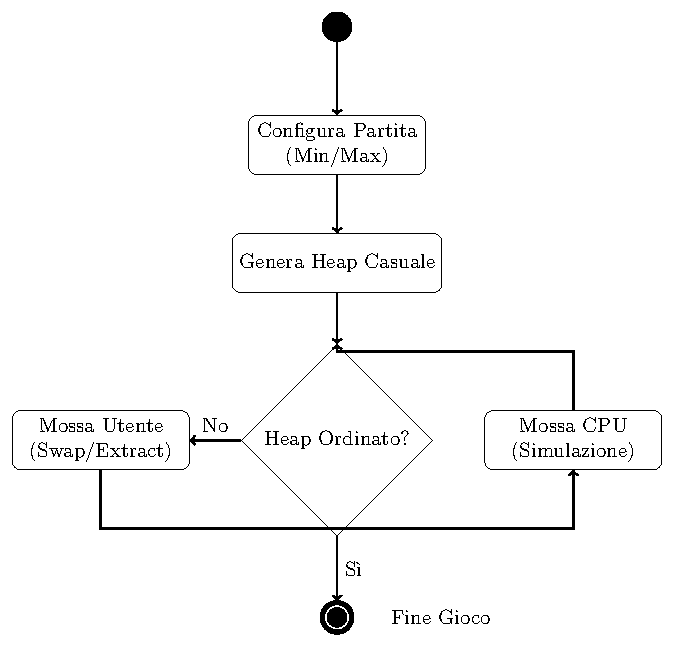
\includegraphics[width=0.8\textwidth]{Diagrams/ActivityDiagram_new.pdf}
    \caption{Diagramma delle Attività - Flusso di Gioco}
    \label{fig:activity_main}
\end{figure}

Il flusso inizia con il \textbf{nodo iniziale} (cerchio pieno). L'utente configura la modalità e il sistema inizializza l'ambiente. Successivamente si entra nel \textbf{loop di gioco} (Decision Diamond): finché l'heap non è completamente ordinato, il controllo passa alternativamente all'Utente e alla CPU. Quando la condizione \texttt{heapSize == 0}  soddisfatta, il flusso termina nel \textbf{nodo finale} (cerchio bordato).

\subsection{Dettaglio del Flusso Principale}
Per garantire una corretta esecuzione dell'algoritmo e un'esperienza utente fluida, l'applicazione implementa il seguente workflow dettagliato:

\begin{enumerate}
    \item \textbf{Fase di Configurazione (Setup)}
    \begin{itemize}
        \item L'utente seleziona la modalità di ordinamento desiderata (\textit{Min-Heap} o \textit{Max-Heap}) tramite l'interfaccia.
        \item Il sistema inibisce i controlli di gioco finché non viene premuto il pulsante di avvio.
    \end{itemize}

    \item \textbf{Fase di Inizializzazione}
    \begin{itemize}
        \item Alla pressione di "Start Game", il sistema genera un array di 15 numeri interi pseudo-casuali (range 1-99).
        \item Viene costruita la struttura ad albero binario visuale corrispondente all'array disordinato.
        \item Il timer di gioco viene avviato.
    \end{itemize}

    \item \textbf{Core Loop (Ciclo di Gioco)}
    \begin{itemize}
        \item \textit{Turno Utente}: L'utente deve identificare e correggere le violazioni della proprietà di heap. Seleziona un nodo padre e un figlio; se lo scambio è valido (cio rispetta l'algoritmo), il sistema anima lo spostamento nodale.
        \item \textit{Validazione Continua}: Dopo ogni mossa, il sistema verifica se la radice è un estremo valido (minimo o massimo globale). In caso affermativo, la radice viene estratta automaticamente e spostata nella lista ordinata.
        \item \textit{Turno CPU}: Se la modalità competitiva è attiva, la CPU esegue la sua mossa immediatamente dopo l'utente, simulando un "tempo di ragionamento" per realismo.
    \end{itemize}

    \item \textbf{Fase di Terminazione}
    \begin{itemize}
        \item Il ciclo continua finché l'heap non è vuoto (\texttt{heapSize = 0}).
        \item Il sistema confronta le metriche di performance (numero di mosse) tra Utente e CPU.
        \item Viene mostrato un modale di riepilogo con l'esito della partita (Vittoria/Sconfitta) e le statistiche dettagliate.
    \end{itemize}
\end{enumerate}

\section{Diagramma delle Classi}
Il Diagramma delle Classi (Class Diagram)  un diagramma strutturale UML che descrive l'architettura del sistema rappresentando le classi, i loro attributi, i metodi e le relazioni tra oggetti. È fondamentale per la progettazione orientata agli oggetti (OOP) in quanto mappa direttamente l'implementazione del codice, fungendo da "blueprint" per lo sviluppo software.

\begin{figure}[ht!]
    \centering
    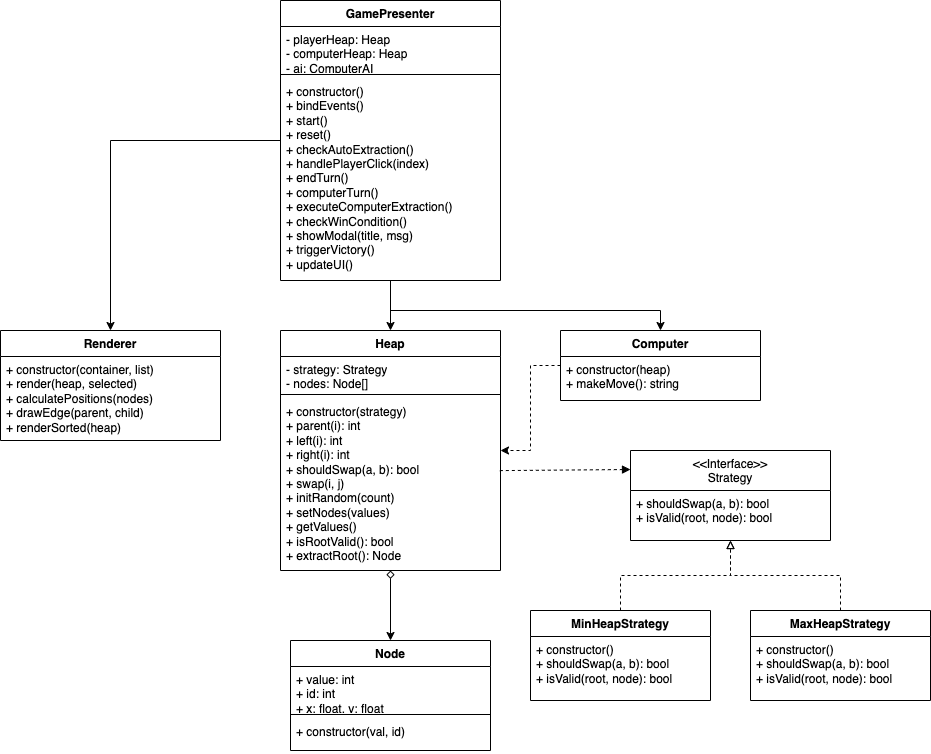
\includegraphics[width=0.9\textwidth]{Diagrams/ClassDiagram.png}
    \caption{Diagramma delle Classi - Architettura MVP}
    \label{fig:class_diagram}
\end{figure}

Nel dettaglio dell'applicazione "Heap Sort Challenge", il diagramma evidenzia l'adozione del pattern architettonale \textbf{Model-View-Presenter (MVP)} per separare la logica di business dalla rappresentazione visiva. Di seguito vengono analizzate in profondità le componenti principali:

\subsection{GamePresenter}
La classe \texttt{GamePresenter} funge da "orchestratore" dell'intera applicazione. Situata nel layer di presentazione, essa media le comunicazioni tra il modello dati (Heap) e la vista (Renderer), garantendo che la logica di gioco rimanga disaccoppiata dall'interfaccia utente.

\subsubsection*{Responsabilità Principali}
\begin{itemize}
    \item \textbf{Gestione del Ciclo di Vita}: Inizializza le istanze di gioco (\texttt{start()}), gestisce il reset (\texttt{reset()}) e monitora lo stato della partita (\texttt{isPlaying}, \texttt{isComputerTurn}).
    \item \textbf{Gestione Eventi}: Tramite il metodo \texttt{bindEvents()}, intercetta le azioni dell'utente (click sui nodi, pulsanti di controllo) e le traduce in comandi per il modello.
    \item \textbf{Coordinamento Turni}: Alterna i turni tra Utente e CPU. Quando l'utente completa una mossa, il presenter invoca \texttt{computerTurn()} dopo un delay artificiale per migliorare l'esperienza utente.
    \item \textbf{Validazione e Feedback}: Verifica se le mosse dell'utente sono lecite (es. scambio padre-figlio) e fornisce feedback visivo immediato tramite il Renderer.
\end{itemize}

\subsubsection*{Metodi Chiave}
\begin{description}
    \item[\texttt{start()}] Configura una nuova partita istanziando gli Heap con la strategia selezionata (Min o Max). Genera i dati casuali e avvia il timer.
    \item[\texttt{handlePlayerClick(index)}] Gestisce la logica di selezione multipla. Mantiene un array \texttt{selectedIndices}; quando due nodi sono selezionati, verifica la relazione di parentela e tenta lo scambio.
    \item[\texttt{checkAutoExtraction()}] Verifica se la radice dell'heap soddisfa la proprietà di ordinamento. In caso positivo, scatena l'estrazione automatica e incrementa il contatore delle mosse.
    \item[\texttt{checkWinCondition()}] Confronta la dimensione degli heap di giocatore e computer. Se uno dei due è vuoto, determina il vincitore basandosi sul numero di mosse e mostra il modale di fine partita.
\end{description}

\subsection{Heap}
La classe \texttt{Heap} incapsula la struttura dati e la logica algoritmica. È il cuore matematico dell'applicazione, responsabile del mantenimento della "Heap Property".

\subsubsection*{Design Pattern: Strategy}
Per supportare sia Min-Heap che Max-Heap senza duplicare il codice, la classe \texttt{Heap} utilizza il \textbf{Strategy Pattern}. Al momento dell'istanziazione, riceve un oggetto che implementa l'interfaccia \texttt{Strategy} (con metodi \texttt{shouldSwap} e \texttt{isValid}). Questo permette all'Heap di delegare la logica di confronto, rimanendo agnostico rispetto al tipo di ordinamento specifico.

\subsubsection*{Attributi e Struttura}
\begin{itemize}
    \item \texttt{nodes}: Un array dinamico di oggetti \texttt{Node}. Rappresenta l'albero binario completo, dove per un nodo all'indice $i$, i figli si trovano a $2i+1$ e $2i+2$.
    \item \texttt{strategy}: Riferimento all'istanza della strategia corrente (\texttt{MinHeapStrategy} o \texttt{MaxHeapStrategy}).
    \item \texttt{sorted}: Array che raccoglie gli elementi mano a mano che vengono estratti dalla radice, formando la lista ordinata finale.
\end{itemize}

\subsubsection*{Metodi Chiave}
\begin{description}
    \item[\texttt{initRandom(count)}] Popola l'heap con $N$ numeri interi unici generati pseudo-casualmente. Garantisce che non ci siano duplicati per semplificare l'apprendimento.
    \item[\texttt{swap(i, j)}] Esegue lo scambio fisico di due nodi nell'array interno. È l'operazione atomica fondamentale dell'algoritmo.
    \item[\texttt{isRootValid()}] Scansiona linearmente l'heap per verificare se la radice è l'estremo globale (minimo o massimo) rispetto a tutti gli altri nodi. Utilizza \texttt{strategy.isValid()}.
    \item[\texttt{extractRoot()}] Rimuove la radice, sposta l'ultimo elemento in cima (o gestisce il caso di heap vuoto) e restituisce il nodo estratto per l'inserimento nella lista ordinata.
\end{description}

% Continues from previous chunk...

\subsection{Renderer}
La classe \texttt{Renderer}  responsabile della rappresentazione grafica dello stato del gioco. Disaccoppiata dalla logica di business, si limita a riflettere visivamente i dati forniti dal Model, gestendo il Document Object Model (DOM) del browser.

\subsubsection*{Rendering Dinamico}
Il rendering avviene in due fasi: calcolo posizionale e disegno.
\begin{itemize}
    \item \textbf{Algoritmo di Posizionamento}: Per rappresentare l'heap come un albero binario bilanciato, il renderer calcola le coordinate $(x, y)$ di ogni nodo. La larghezza disponibile viene suddivisa ricorsivamente in base alla profondità del nodo, garantendo che l'albero si adatti dinamicamente al container HTML.
    \item \textbf{Gestione DOM}: Utilizza elementi HTML standard (div) per disegnare nodi e archi. Ogni volta che lo stato cambia (es. dopo uno swap), il renderer ridisegna le connessioni ma ottimizza l'aggiornamento dei nodi esistenti per permettere animazioni CSS fluide (transizioni di posizione).
\end{itemize}

\subsubsection*{Metodi Chiave}
\begin{description}
    \item[\texttt{render(heap, selectedIndices)}] Metodo principale invocato dal Presenter. Riceve l'oggetto Heap completo e la lista degli indici selezionati.
    \item[\texttt{calculatePositions(nodes)}] Assegna le coordinate spaziali ad ogni nodo. Il livello $L$ determina la coordinata $Y$, mentre la posizione nell'array determina l'offset $X$.
    \item[\texttt{drawEdge(parent, child)}] Utilizza CSS transforms per tracciare una linea di connessione tra due nodi, aggiornandola dinamicamente durante le animazioni.
    \item[\texttt{renderSorted(heap)}] Visualizza separatamente l'array \texttt{sorted}, mostrando all'utente i "frutti" del lavoro di ordinamento (es. i numeri estratti in ordine crescente o decrescente).
\end{description}

\subsection{Computer}
La classe \texttt{Computer} implementa la logica dell'avversario. Nonostante sia un'applicazione educativa, il computer deve simulare un comportamento "competente" per fornire una sfida.

\subsubsection*{Logica Decisionale}
Il computer opera su una propria istanza di \texttt{Heap}, speculare a quella del giocatore all'inizio.
\begin{enumerate}
    \item \textbf{Priorità all'Estrazione}: Il metodo \texttt{makeMove()} controlla prima di tutto se la radice è valida (\texttt{isRootValid()}). Se lo è, il computer "attende" il prossimo ciclo per estrarre, massimizzando il punteggio.
    \item \textbf{Strategia di Correzione}: Se la radice non è pronta, il computer cerca attivamente violazioni della proprietà di heap. Scansiona l'albero per trovare nodi che violano la regola rispetto ai propri figli e propone uno scambio correttivo.
    \item \textbf{Simulazione Umana}: Introduce ritardi artificiali per rendere le mosse visibili e comprensibili all'utente, evitando che il computer completi il gioco istantaneamente.
\end{enumerate}

\subsection{Node}
La classe \texttt{Node}  una struttura dati semplice (POJO - Plain Old JavaScript Object) che funge da contenitore di informazioni.
\begin{itemize}
    \item \texttt{value}: Il valore numerico intero da ordinare.
    \item \texttt{id}: Un identificativo univoco per tracciare l'elemento nel DOM durante i ri-ordinamenti, essenziale per le animazioni (chiave di riconciliazione).
    \item \texttt{x, y}: Coordinate calcolate dal Renderer, memorizzate nel nodo per evitare ricalcoli costanti durante un singolo frame di rendering.
\end{itemize}

\subsection{Interfaccia Strategy}
Il pattern Strategy è cruciale per la flessibilità del gioco.
\begin{itemize}
    \item \textbf{MinHeapStrategy}: Implementa \texttt{shouldSwap(a, b)} restituendo \texttt{true} se $a > b$ (il padre è maggiore del figlio, violazione Min-Heap). Implementa \texttt{isValid} verificando $parent \leq child$.
    \item \textbf{MaxHeapStrategy}: Inverte la logica, restituendo \texttt{shouldSwap = true} se $a < b$.
\end{itemize}
Questa astrazione permette di cambiare la modalità di gioco (dal "Min Heap" al "Max Heap") iniettando semplicemente una diversa istanza di strategia nel costruttore dell'Heap, senza modificare una riga della logica centrale dell'Heap stesso.

\section{Diagramma di Sequenza}
Il Diagramma di Sequenza (Sequence Diagram)  un diagramma di interazione UML che illustra come gli oggetti collaborano in un determinato scenario, ponendo l'accento sull'ordine temporale dei messaggi scambiati. A differenza del Diagramma delle Classi (statico) o del Diagramma delle Attività (flusso di lavoro), il Diagramma di Sequenza cattura la dinamica "runtime" del sistema.

Nel contesto di questa applicazione, l'adozione dei Diagrammi di Sequenza è fondamentale per documentare e comprendere due aspetti critici che non emergono dagli altri diagrammi:
\begin{itemize}
    \item \textbf{Il Flusso MVP}: Visualizza chiaramente il percorso "round-trip" di un'azione. Ad esempio, un click dell'utente (View) viene intercettato dal Presenter, che interroga il Model, applica la logica di business, e infine comanda alla View di aggiornarsi. Questo assicura che il principio di "Separation of Concerns" sia rispettato rigorosamente.
    \item \textbf{Gestione Temporale e Animazioni}: L'applicazione utilizza transizioni visive per mostrare gli scambi e introduce ritardi funzionali durante il turno dell'avversario per migliorare la comprensione dell'algoritmo. Il diagramma esplicita come il sistema coordini questi eventi asincroni, assicurando che l'aggiornamento dello stato logico avvenga solo al termine delle animazioni, garantendo così la coerenza visiva.
\end{itemize}
L'utilizzo di questo diagramma ci permette di verificare la correttezza della logica di coordinamento, specialmente nelle fasi più complesse come l'estrazione ricorsiva della radice o il turno automatizzato del computer.


\subsection{Sequenza Principale del Gioco}

\begin{figure}[H]
    \centering
    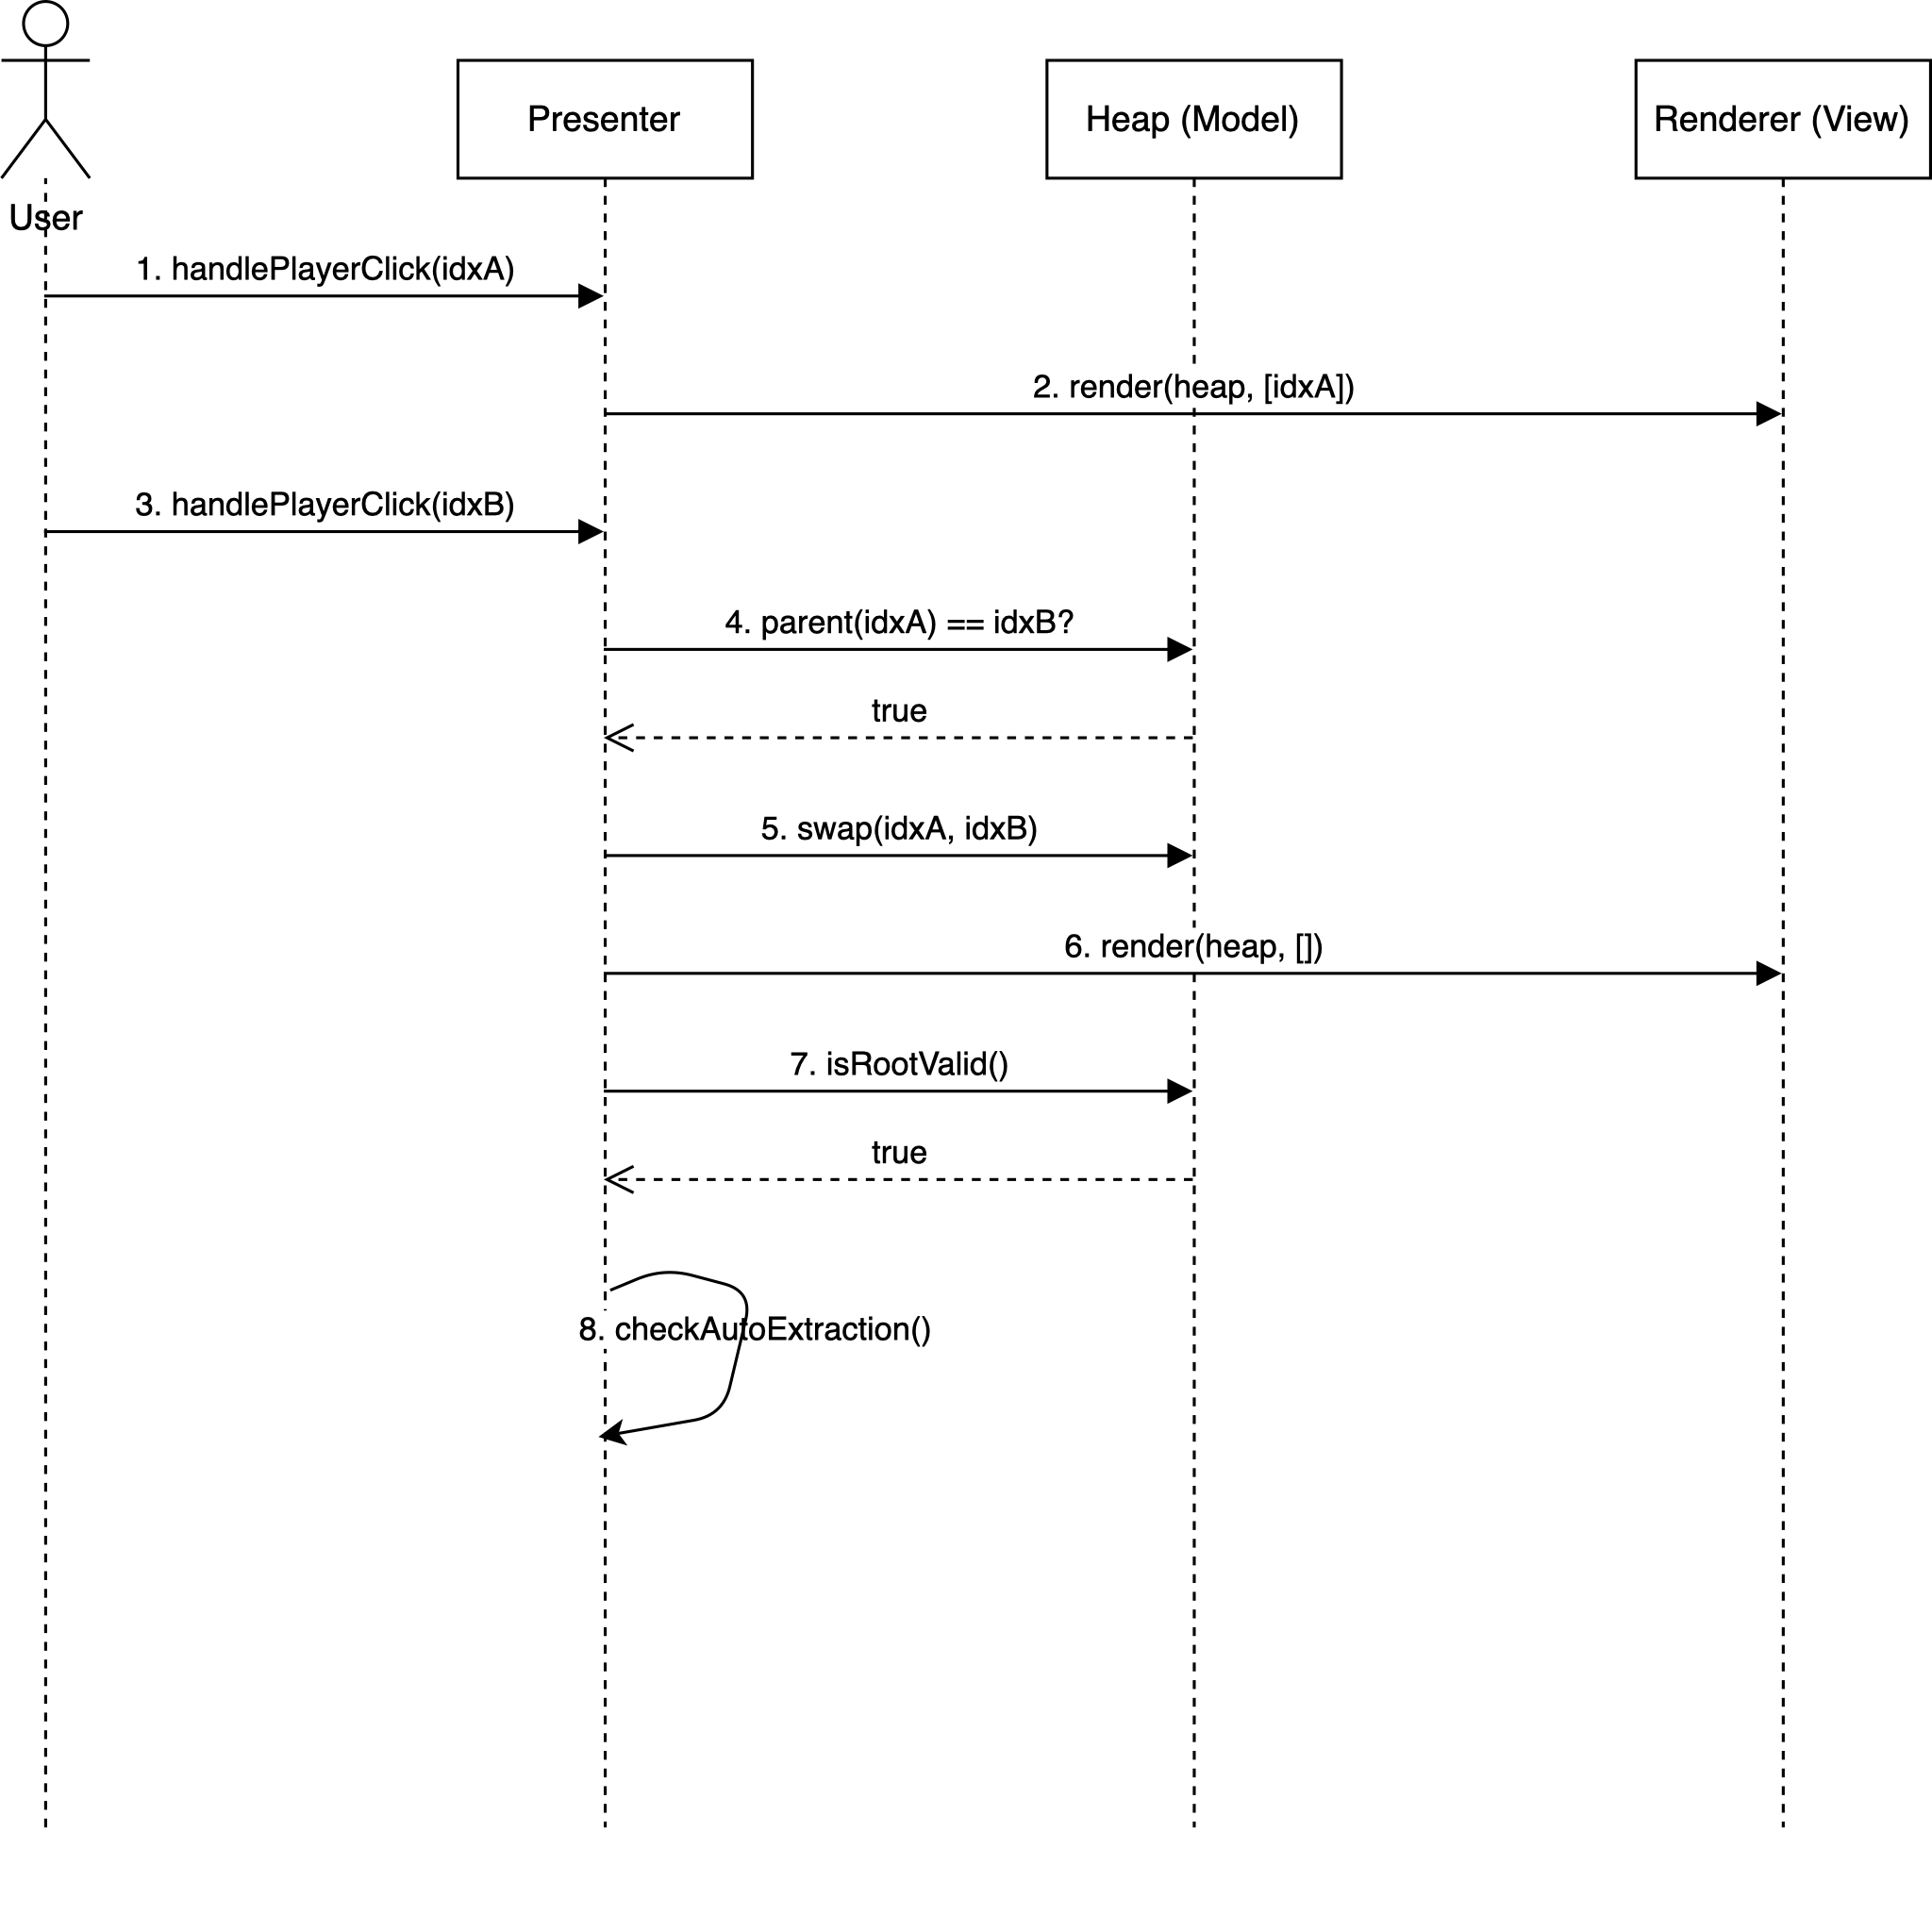
\includegraphics[width=0.95\textwidth]{Diagrams/sequenceDiagram1.png}
    \caption{Diagramma di Sequenza - Scenario: Selezione e Swap Utente}
    \label{fig:sequence_diagram}
\end{figure}


Il diagramma di sequenza in Figura \ref{fig:sequence_diagram} descrive dettagliatamente il flusso di interazione durante una mossa di gioco, specificamente lo scambio (\texttt{swap}) tra due nodi deciso dall'utente.
Questa operazione, apparentemente semplice, innesca una catena complessa di eventi che attraversa tutti i livelli dell'architettura MVP.

Di seguito analizziamo nel dettaglio le fasi che compongono questo scenario:

\phantomsection
\subsubsection{Gestione degli Eventi e Selezione}
Tutto ha inizio nel livello della Vista (\texttt{Renderer}).
L'applicazione implementa il pattern \textbf{Event Delegation}: invece di attaccare un listener a ogni singolo nodo (che sarebbe dispendioso in termini di memoria), un unico event listener è collegato al contenitore padre dell'albero.
Quando l'utente clicca su un nodo (identificato come \texttt{idxA}):
\begin{itemize}
    \item L'evento \texttt{click} risale il DOM fino al contenitore.
    \item Il \texttt{Renderer} estrae l'ID del nodo target dall'attributo \texttt{data-index}.
    \item Il controllo viene passato al \texttt{GamePresenter} tramite il metodo \texttt{handlePlayerClick(idxA)}.
\end{itemize}

Il Presenter mantiene lo stato della selezione interna.
Se è il primo click, il nodo viene semplicemente marcato come "selezionato" e il Renderer viene istruito di evidenziarlo visivamente (cambio di colore e spessore del bordo).
Il diagramma si concentra sul caso del \textbf{secondo click} (\texttt{idxB}), che innesca il tentativo di mossa.

\phantomsection
\subsubsection{Validazione Logica}
Prima di modificare qualsiasi dato, il sistema deve garantire l'integrità delle regole del gioco.
Il \texttt{Presenter} interroga il \texttt{Model} (\texttt{Heap}) per validare la mossa:
\begin{enumerate}
    \item \textbf{Adiacenza}: I due nodi devono essere adiacenti nell'albero (padre-figlio). La formula matematica $parent = \lfloor (child - 1) / 2 \rfloor$ permette una verifica istantanea $O(1)$.
    \item \textbf{Proprietà di Heap}: Non basta che i nodi siano vicini; il loro scambio deve essere "utile".
    \begin{itemize}
        \item In un \textit{Max-Heap}, se il figlio è maggiore del padre ($A[child] > A[parent]$), lo scambio è necessario.
        \item In un \textit{Min-Heap}, se il figlio è minore del padre ($A[child] < A[parent]$), lo scambio è necessario.
    \end{itemize}
\end{enumerate}
Questa logica di validazione è incapsulata nel metodo \texttt{shouldSwap()} della Strategy attiva. Se la validazione fallisce, il Presenter innesca un feedback di errore (animazione "shake") e resetta la selezione senza toccare il Modello.

\phantomsection
\subsubsection{Manipolazione dei Dati e Coerenza}
Se la validazione ha successo (il percorso marcato come \texttt{true} nel diagramma), il Presenter invoca il comando \texttt{swap(idxA, idxB)} sul Modello.
Questa è un'operazione critica che modifica lo stato persistente dell'applicazione:
\begin{itemize}
    \item L'array sottostante viene aggiornato: i valori alle posizioni $A$ e $B$ vengono scambiati.
    \item Gli oggetti \texttt{Node} mantengono i loro ID univoci ma cambiano posizione nell'array. Questo è fondamentale per permettere al framework di rendering di tracciare l'identità degli elementi (Object Identity) e animarli correttamente.
\end{itemize}

\phantomsection
\subsubsection{Riconciliazione della Vista}
Una volta mutato il Modello, la Vista deve essere sincronizzata.
Invece di ridisegnare tutto l'albero da zero (che causerebbe un "flash" sgradevole e la perdita del contesto visivo), il sistema adotta un approccio differenziale:
\begin{itemize}
    \item Il Presenter chiama \texttt{render(heap)}.
    \item Il \texttt{Renderer} calcola le nuove coordinate $(x, y)$ target per ogni nodo.
    \item Poiché i nodi DOM hanno un ID stabile, il browser può interpolare la posizione vecchia e quella nuova.
    \item Viene applicata una transizione CSS (\texttt{transition: transform 0.5s}).
\end{itemize}
Durante questa fase di animazione, l'input utente viene temporaneamente disabilitato per evitare "Race Conditions" (es. l'utente clicca su un nodo che si sta muovendo).

\phantomsection
\subsubsection{Verifica Post-Mossa e Automazione}
Il diagramma termina con una fase di verifica globale (\texttt{isRootValid} e \texttt{checkAutoExtraction}).
Dopo uno scambio, la nuova configurazione potrebbe aver sbloccato nuove possibilità:
\begin{itemize}
    \item La radice potrebbe essere diventata il massimo/minimo assoluto. In tal caso, il sistema deve procedere all'estrazione automatica.
    \item Potrebbero essersi create nuove violazioni a cascata nei sotto-alberi (anche se nel caso del giocatore singolo, le mosse sono puntuali).
\end{itemize}
Se la radice è valida, il Presenter scatena l'evento di estrazione, che a sua volta generer è un nuovo ciclo di aggiornamenti (rimozione nodo, spostamento ultimo elemento, nuova fase di heapify), dimostrando la natura ricorsiva e ciclica dell'algoritmo Heap Sort.

In sintesi, la Figura \ref{fig:sequence_diagram} non mostra solo uno "spostamento di numeri", ma la coreografia precisa tra input asincrono dell'utente, validazione sincrona della logica matematica e rendering differito per l'esperienza utente.




\subsection{Interazione tra Classi - Turno Computer}
Il diagramma seguente (Figura \ref{fig:class_comm}) illustra le interazioni tra le componenti del sistema durante il turno del Computer.

\begin{figure}[H]
    \centering
    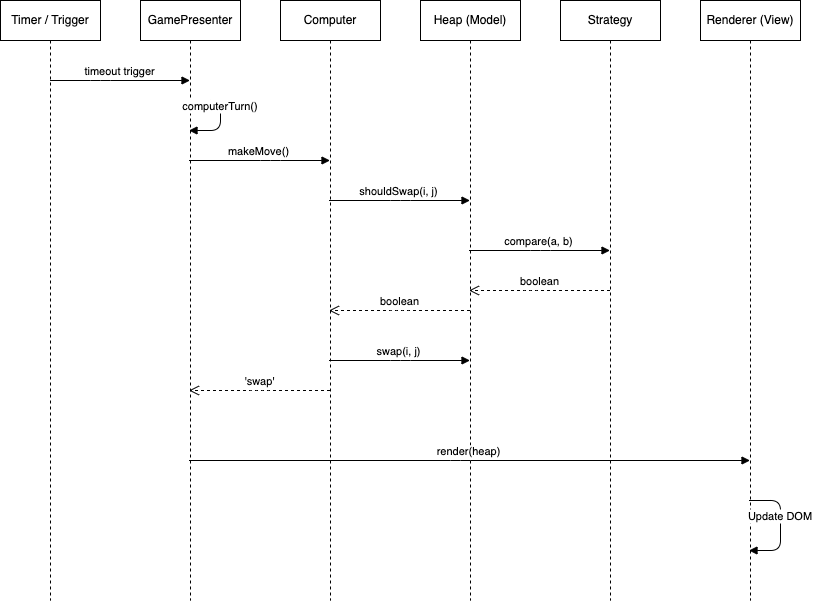
\includegraphics[width=0.95\textwidth]{Diagrams/ClassCommunication.png}
    \caption{Diagramma di Sequenza - Comunicazione tra Classi (Turno Computer)}
    \label{fig:class_comm}
\end{figure}



Il flusso di esecuzione delle operazioni durante il turno del Computer, rappresentato nella Figura \ref{fig:class_comm},  un esempio paradigmatico di come un'architettura Model-View-Presenter possa gestire la logica asincrona e algoritmica senza compromettere la fluidità dell'interfaccia. Di seguito viene presentata un'analisi tecnica approfondita, suddivisa in fasi logiche che mappano gli 11 passaggi del diagramma.

\phantomsection
\subsubsection{Orchestrazione Temporale e Infinesco}
A differenza del turno del giocatore, che è guidato da input diretti (click), il turno del computer è un processo \textbf{time-driven}. 
Tutto ha inizio con un'interazione tra un timer asincrono (\texttt{setTimeout}) e il \texttt{GamePresenter}:
\begin{itemize}
    \item \textbf{Decoupling}: L'invocazione di \texttt{computerTurn()} avviene dopo un ritardo variabile (tipicamente 1000-1500ms). Questo è fondamentale per la User Experience, poiché permette all'utente di "vedere" il computer che pensa, evitando un'esecuzione istantanea che risulterebbe confusionaria.
    \item \textbf{State Management}: Il Presenter imposta internamente il flag \texttt{isComputerTurn} a \texttt{true}. Questo blocca temporaneamente gli input del giocatore, prevenendo "Race Conditions" dove l'utente e il computer potrebbero tentare di modificare lo stesso Heap contemporaneamente.
\end{itemize}

\phantomsection
\subsubsection{Analisi Strategica e Scansione del Modello}
Ricevuto il comando dal Presenter (\texttt{makeMove()}), la classe \texttt{Computer} inizia la fase di analisi. Il computer non "vede" l'interfaccia grafica; esso interagisce esclusivamente con l'interfaccia pubblica del Modello (\texttt{Heap}):
\begin{itemize}
    \item \textbf{Ricerca di Violazioni}: Il computer scansiona l'array dello heap cercando la prima coppia di nodi (padre-figlio) che viola la proprietà fondamentale dell'algoritmo (es. un padre più piccolo di un figlio in un Max-Heap).
    \item \textbf{Agnosticismo dei Dati}: Il computer non sa se sta giocando con un Min-Heap o un Max-Heap. Esso si limita a chiedere allo Heap: \texttt{shouldSwap(parent, child)}. Questa astrazione è il primo livello di difesa contro la duplicazione del codice.
\end{itemize}

\phantomsection
\subsubsection{Il Pattern Strategy in Azione}
Il diagramma evidenzia il ruolo cruciale del \textbf{Pattern Strategy} (passaggi 5 e 6). Lo \texttt{Heap} riceve la richiesta di validazione dal Computer e la delega immediatamente alla strategia attiva:
\begin{itemize}
    \item \textbf{Delegazione Pura}: Lo \texttt{Heap} possiede un riferimento a un'interfaccia \texttt{Strategy}. Se la strategia  \texttt{MinHeapStrategy}, il confronto restituir  \texttt{true} se il figlio è minore del padre. Se  \texttt{MaxHeapStrategy}, la logica sarà opposta.
    \item \textbf{Separazione delle Preoccupazioni}: Questa fase dimostra come la logica matematica pura sia isolata dalla struttura dati. Lo Heap gestisce l'albero (posizioni, indici), mentre la Strategy gestisce la verità matematica (confronto).
\end{itemize}

\phantomsection
\subsubsection{Esecuzione della Mutazione e Integrità del Modello}
Una volta ottenuta la conferma (\texttt{boolean: true}), il Computer passa all'azione (passaggio 8). Invocando \texttt{swap(i, j)}, il computer modifica lo stato interno del sistema:
\begin{itemize}
    \item \textbf{Atomicit }: Lo scambio dei valori nell'array è un'operazione atomica che garantisce che il Modello sia sempre in uno stato consistente prima di passare alla fase successiva.
    \item \textbf{Preservazione dell'Identità}: Nonostante i valori vengano scambiati, gli oggetti \texttt{Node} coinvolti mantengono il loro ID univoco. Questo permetter è successivamente al Renderer di tracciare il movimento "fisico" del nodo sullo schermo invece di limitarsi a cambiare un testo.
\end{itemize}

\phantomsection
\subsubsection{Feedback Loop e Ritorno del Controllo}
Terminata la mossa, il Computer restituisce un segnale al Presenter (passaggio 9). Questo passaggio è vitale per la comunicazione inter-livello:
\begin{itemize}
    \item \textbf{Signal Handling}: Il ritorno della stringa \texttt{'swap'} comunica al Presenter che un'azione è stata effettivamente compiuta e che è necessario un aggiornamento visivo.
    \item \textbf{Analisi Post-Mossa}: Se il computer non avesse trovato mosse valide, avrebbe restituito un valore diverso (es. \texttt{'no-move'}), indicando al Presenter che il turno del computer è terminato o che è necessaria un'estrazione.
\end{itemize}

\phantomsection
\subsubsection{Sincronizzazione della Vista e Rendering Differenziale}
L'ultima fase del diagramma descrive il passaggio dal dato logico all'immagine visiva:
\begin{enumerate}
    \item \textbf{Comando di Rendering}: Il Presenter chiama \texttt{render(heap)}. È importante notare che il Presenter passa l'intero stato dello Heap alla Vista, mantenendo la Vista "stupida": essa non deve calcolare cosa è successo, ma solo "dipingere" lo stato attuale.
    \item \textbf{Ottimizzazione del DOM}: Il \texttt{Renderer} calcola le nuove coordinate $(x, y)$ per i nodi modificati. Grazie alla persistenza degli ID degli elementi DOM, il CSS può applicare transizioni fluide tra le vecchie coordinate e le nuove, creando l'illusione di un movimento fluido che aiuta l'apprendimento dell'utente.
\end{enumerate}

\phantomsection
\subsubsection{Considerazioni Finali sul Flusso Computer}
In conclusione, la densità di messaggi mostrata in Figura \ref{fig:class_comm} riflette la robustezza dell'architettura. Suddividere il turno del computer in 11 passaggi permette di:
\begin{itemize}
    \item \textbf{Testability}: Ogni passaggio (validazione, scambio, rendering) può essere testato unitariamente.
    \item \textbf{Scalability}: È possibile aggiungere nuove strategie di gioco o nuovi tipi di computer (es. un computer "difficile") semplicemente implementando nuove sottoclassi di \texttt{Computer} o \texttt{Strategy}, senza mai toccare il codice del Presenter o del Renderer.
\end{itemize}
Il risultato finale è un sistema dove la "macchina" gioca contro l'utente seguendo le stesse rigide regole matematiche, garantendo un'esperienza educativa coerente e priva di errori logici.


\section{Diagramma dei Componenti}
Il diagramma dei componenti illustra l'organizzazione logico-funzionale del sistema, evidenziando la scomposizione dell'applicazione in moduli indipendenti e la loro strutturazione in livelli (layers). Questa visione architetturale permette di comprendere come le diverse parti del software collaborino per fornire un'esperienza utente coerente e performante.

L'applicazione segue un'architettura a tre livelli (\textit{Three-Tier Architecture}), dove ogni layer ha responsabilità ben definite e comunica con gli altri tramite interfacce standardizzate.

\begin{figure}[H]
    \centering
    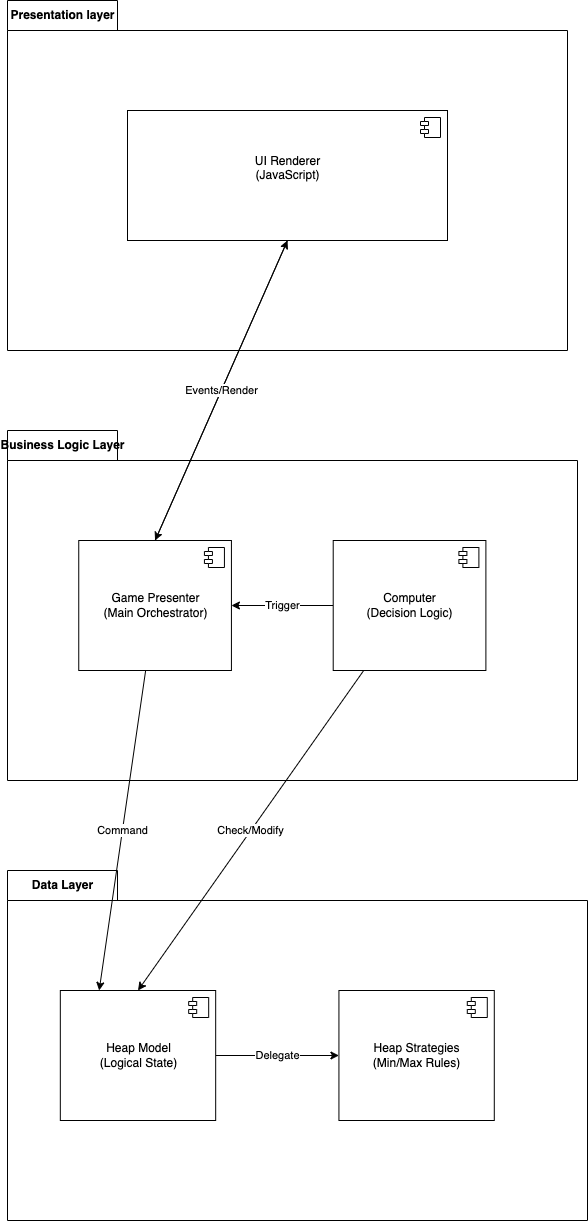
\includegraphics[width=0.92\textwidth,height=0.60\textheight,keepaspectratio]{Diagrams/ComponentDiagram.png}
    \caption{Diagramma dei Componenti - Architettura Three-Tier}
    \label{fig:component_diagram}
\end{figure}

Di seguito viene riportata una descrizione dettagliata dei tre livelli rappresentati in Figura \ref{fig:component_diagram}:

\phantomsection
\subsection{Presentation Layer}
Questo livello costituisce la "pelle" dell'applicazione, gestendo l'interazione diretta con l'utente finale.
\begin{itemize}
    \item \textbf{UI Renderer}: È il modulo incaricato di tradurre lo stato logico in elementi grafici. Utilizza tecniche di manipolazione del DOM per visualizzare l'albero binario e gestire le transizioni fluide durante gli scambi di nodi.
    \item \textbf{Styles \& Assets}: Definisce l'estetica del software tramite CSS3 (utilizzando Flexbox e Grid) e la struttura portante tramite HTML5 semantico.
\end{itemize}

\phantomsection
\subsection{Business Logic Layer}
Situato al centro dell'architettura, questo layer coordina il flusso dei dati e le regole del gioco.
\begin{itemize}
    \item \textbf{Game Presenter}: Funge da mediatore tra la Vista e il Modello (pattern MVP). Gestisce la coda degli eventi, il calcolo del punteggio e la sincronizzazione dei turni.
    \item \textbf{Computer Engine}: Un modulo specializzato che isola la logica decisionale dell'avversario virtuale. Esso analizza lo stato dello heap e determina la mossa ottimale basandosi sulla strategia corrente.
\end{itemize}

\phantomsection
\subsection{Data Layer}
Sebbene l'applicazione non utilizzi un database persistente esterno, il Data Layer gestisce la persistenza in-memory e l'integrità algoritmica.
\begin{itemize}
    \item \textbf{Heap Model}: La componente che custodisce l'array dei nodi. Implementa le operazioni matematiche di \textit{sift-up} e \textit{sift-down}, garantendo che lo stato interno sia sempre coerente.
    \item \textbf{Strategies}: Rappresenta l'astrazione delle regole di confronto (Pattern Strategy). Questo componente permette di trasformare istantaneamente il comportamento di tutto l'albero da Min-Heap a Max-Heap senza riavviare l'applicazione.
\end{itemize}


\newpage
\section{Architettura del Progetto}
L'architettura proposta per il sistema è stata progettata seguendo i principi del pattern Model-View-Presenter (MVP), con l'obiettivo di garantire una netta separazione delle responsabilità e facilitare la manutenibilità futura.

La Figura \ref{fig:layered_architecture} presenta lo schema logico di questa suddivisione a livelli, definendo le interazioni previste tra l'interfaccia utente (View), la logica di controllo (Presenter) e la gestione dei dati (Model).

A supporto di questa architettura, la Figura \ref{fig:dir_structure} propone l'organizzazione strutturale delle directory, dettagliando come i vari componenti logici verranno mappati nel file system:


\noindent\textbf{Schema dell'Architettura Model-View-Presenter:}

\begin{figure}[H]
\centering
\scalebox{0.85}{
\begin{tikzpicture}[
    node distance=0cm,
    layer/.style={
        rectangle,
        draw=black,
        minimum width=12cm,
        minimum height=2.0cm,
        text width=2.5cm,
        align=center,
        font=\bfseries,
        anchor=north west
    },
    component/.style={
        rectangle,
        draw=black,
        fill=white,
        minimum width=3cm,
        minimum height=1.0cm,
        align=center,
        font=\small,
        rounded corners
    }
]

    % --- LAYERS ---
    % 1. View Layer (Yellow)
    \node [layer, fill=yellow!30] (presentation) at (0,0) {View Layer \\ (Presentation)};
    
    % 2. Presenter Layer (Green)
    \node [layer, fill=green!30] (business) at (0,-2.0) {Presenter Layer \\ (Business Logic)};
    
    % 3. Model Layer (Blue)
    \node [layer, fill=blue!30] (data) at (0,-4.0) {Model Layer \\ (Data \& State)};


    % --- COMPONENTS ---
    
    % Presentation Components (Far Right)
    \node [component] (renderer) at (10.5, -1.0) {Renderer.js \\ (View)};
    
    % Business Logic Components (Presenter Far Left)
    \node [component] (presenter) at (3.0, -3.0) {GamePresenter.js \\ (Presenter)};
    \node [component] (computer) at (9.0, -3.0) {Computer.js \\ (Engine)};
    
    % Data Components (Right)
    \node [component] (heap) at (9.0, -5.0) {Heap.js \\ (Model)};


    % --- ARROWS ---
    % View <-> Presenter
    \draw [-latex, thick] (renderer.south) -- ++(0,-0.4) -| (presenter.north);
    \draw [-latex, thick] (presenter.north) |- ++(0,0.4) -| (renderer.south);
    
    % Presenter -> Model
    \draw [-latex, thick] (presenter.south) -- ++(0,-0.4) -| (heap.north);
    \draw [-latex, thick] (heap.north) |- ++(0,0.4) -| (presenter.south);
    
    % Computer -> Heap
    \draw [-latex, thick] (computer.south) -- ++(0,-0.4) -| (heap.north);

    % Presenter <-> Computer
    \draw [-latex, thick] (presenter.east) -- (computer.west);

\end{tikzpicture}
}
\caption{Diagramma Architetturale a Livelli (Layered Architecture)}
\label{fig:layered_architecture}
\end{figure}

\noindent\textbf{Struttura delle Directory:}

\begin{figure}[H]
\centering
\begin{minipage}{0.8\textwidth}
\dirtree{%
.1 src/.
.2 main.js \DTcomment{Entry Point, inizializzazione app}.
.2 style.css \DTcomment{Stili globali e layout}.
.2 Model/ \DTcomment{Logica di Business}.
.3 Heap.js \DTcomment{Struttura dati e algoritmi}.
.3 Node.js \DTcomment{Entità e stato dei nodi}.
.3 Computer.js \DTcomment{AI e decisioni}.
.3 *Strategy.js \DTcomment{Strategie Min/Max}.
.2 View/ \DTcomment{Rappresentazione Visiva}.
.3 Renderer.js \DTcomment{Manipolazione DOM e animazioni}.
.2 Presenter/ \DTcomment{Logica di Controllo}.
.3 GamePresenter.js \DTcomment{Orchestrazione eventi}.
}
\end{minipage}
\caption{Struttura del File System del Progetto}
\label{fig:dir_structure}
\end{figure}

\begin{itemize}
    \item \textbf{src/}: La radice del codice sorgente contiene i moduli principali e il punto di ingresso dell'applicazione.
    \begin{itemize}
        \item \texttt{main.js}: Il punto di ingresso (Entry Point). Inizializza l'applicazione, istanzia le classi principali e avvia il ciclo di vita del software.
        \item \texttt{style.css}: Il foglio di stile globale che definisce il look \& feel, le animazioni e il layout responsivo.
    \end{itemize}
    
    \item \textbf{src/Model/}: Contiene la logica di business e la gestione dei dati.
    \begin{itemize}
        \item \texttt{Heap.js}: La classe che gestisce la struttura dati vera e propria (l'array) e implementa gli algoritmi di ordinamento e mantenimento delle proprietà di heap.
        \item \texttt{Node.js}: Rappresenta la singola entità (nodo) dell'albero, incapsulando il valore e l'identificativo univoco.
        \item \texttt{Computer.js}: Implementa l'intelligenza artificiale dell'avversario.
        \item \texttt{MinHeapStrategy.js} e \texttt{MaxHeapStrategy.js}: Implementazioni concrete delle strategie di confronto (Pattern Strategy).
    \end{itemize}
    
    \item \textbf{src/View/}: Responsabile della rappresentazione visiva.
    \begin{itemize}
        \item \texttt{Renderer.js}: Gestisce la manipolazione del DOM, disegnando l'albero e animando i movimenti dei nodi in risposta ai cambiamenti di stato.
    \end{itemize}
    
    \item \textbf{src/Presenter/}: Il mediatore tra Model e View.
    \begin{itemize}
        \item \texttt{GamePresenter.js}: Il cuore pulsante dell'applicazione. Coordin le interazioni utente, invoca la logica del Modello e aggiorna la Vista.
    \end{itemize}
\end{itemize}

\chapter{Implementazione e Validazione}
In questo capitolo viene analizzata in dettaglio l'implementazione pratica del progetto "Heap Sort Challenge". L'obiettivo è duplice: da un lato descrivere le scelte tecniche e architetturali adottate per la costruzione del software didattico; dall'altro, illustrare analiticamente il comportamento delle strutture dati, l'orchestrazione degli algoritmi e le meccaniche di interazione con l'utente. Attraverso una dissezione tecnica approfondita, verrà spiegata come l'astrazione concettuale del pensiero computazionale sia stata tradotta in codice sorgente funzionale ed efficiente.

\section{Introduzione alle Scelte Tecnologiche}
La realizzazione di un'applicazione web interattiva richiede un'attenta valutazione dello stack tecnologico. Nel panorama moderno dello sviluppo frontend, si assiste spesso all'adozione pervasiva di framework e librerie strutturate (come React, Angular, o Vue) e di astrazioni complesse come TypeScript. Sebbene questi strumenti offrano indiscutibili vantaggi per applicazioni Enterprise di larga scala gestite da team numerosi, per il presente caso di studio si è optato consapevolmente per un approccio diverso: lo sviluppo interamente in \textbf{Vanilla JavaScript (ES6+)}, supportato unicamente da HTML5 e CSS3 nativi, senza alcuna dipendenza esterna (Zero-Dependencies Approach).

Questa scelta architetturale è motivata da diverse ragioni didattiche ed ingegneristiche:
\begin{enumerate}
    \item \textbf{Leggerezza e Accessibilità:} L'applicazione deve essere fruibile da qualsiasi dispositivo (anche mobile o scolastico datato) senza tempi di caricamento dovuti allo scaricamento di voluminose librerie JavaScript. L'assenza di framework abbatte il \textit{bundle size} a pochi kilobyte, garantendo tempi di esecuzione praticamente istantanei.
    \item \textbf{Trasparenza Didattica:} In un progetto focalizzato sull'insegnamento degli algoritmi e delle logiche di programmazione nuda, l'impiego di un framework che astrae pesantemente l'interazione con il \textit{Document Object Model (DOM)} rischierebbe di offuscare la purezza algoritmica. Con Vanilla JS, il flusso di controllo è palese e tracciabile linearmente: dalla logica puramente matematica allo stato visivo finale, non esistono meccanismi "magici" (come il Virtual DOM di React o la digest cycle di AngularJS) a frapporsi.
    \item \textbf{Potenziale Espressivo nativo:} Gli standard moderni di JavaScript (come ECMAScript 6 e versioni successive) hanno introdotto feature native (Classi, Map/Set, Destructuring assignment, Arrow functions, Modules) che colmano in gran parte le lacune architetturali del passato, consentendo lo sviluppo di script perfettamente organizzati, testabili e modulari, in modo totalmente object-oriented, rendendo superflua la sovrascrittura fornita dalle librerie in molti scenari limitati.
\end{enumerate}

Le \textbf{Web API} native (precisamente \texttt{document.createElement}, \texttt{dataset}, \texttt{classList}, \texttt{requestAnimationFrame}) sono risultate sufficienti ed estremamente performanti per la gestione della scacchiera algoritmica che anima questo progetto.

\section{Architettura Model-View-Presenter}
In assenza dell'infrastruttura rigida di un framework, l'intera onere di strutturare logicamente il codice ricade sullo sviluppatore. Affinché il software possieda caratteristiche di \textit{manutenibilità}, \textit{scalabilità} e \textit{basso accoppiamento} (loose coupling), si è deciso di implementare un'architettura rigorosa seguendo il Pattern Architetturale \textbf{Model-View-Presenter (MVP)}, storicamente usato nella costruzione di applicazioni desktop (es. in ambienti Microsoft .NET, Java Swing) ed estremamente efficace in Vanilla JS.

\subsection{Distinzione dal framework MVC}
Sebbene fortemente affine al pattern MVC largamente standardizzato sul web (Specialmente via Back-End), il pattern MVP fornisce una topografia d'interazione \textit{strettamente gerarchica}.
Nel Pattern MVC tradizionale implementato nel frontend, molto spesso la Vista  "attiva": osserva direttamente i cambiamenti di stato emessi dal Modello globale e si ri-renderizza automaticamente.
Al contrario, nell'MVP adottato, la Vista è rigorosamente identificata come \textbf{Passive View}. Il flusso circola esplicitamente come segue:
\begin{enumerate}
    \item L'Utente (Studente) interagisce con il DOM (la Vista).
    \item La Vista non ha intelligenza propria né conoscenza della partita logica; si auto-limita a registrare un click fisico e, passivamente, notifica il \textbf{Presenter}.
    \item Il Presenter incapsula la totale "Business Logic" temporale: interpreta il comando dell'utente, lo traduce in un'istruzione algoritmica (ad esempio: \textit{"E' valido scambiare il nodo di indice 4 col nodo di indice 1 in un Max Heap?"}) e interroga/aggiorna il \textbf{Modello}.
    \item Il Modello, puramente matematico, applica lo scambio (Swap dell'array) e conferma al \textbf{Presenter} il completamento dell'operazione.
    \item Il Presenter riprende il controllo logico e ordina esplicitamente (tramite binding o chiamate procedurali) alla \textbf{Vista} di aggiornare l'interfaccia (eseguire l'animazione di movimento sui DOM element specifici) in totale asincronia ed accoppiamento indiretto.
\end{enumerate}

Questa severa partizione logica (Separation of Concerns) permette per esempio un \textit{Test Unitario} perfetto del Modello: gli algoritmi sui nodi corrono esclusivamente su Array numerici off-screen e Node objects, permettendo in futuro al sorgente model-oriented di servire perfino interfacce testuali o API esterne.

\section{Struttura dei Dati e Logica di Dominio}
Rispettando il pattern MVP, il Livello Modello è l'unico deputato al mantenimento della veridicità e consistenza matematica dell'informazione. Le regole algoritmiche (costruzione, ricerca del minimo/massimo, validazione, estrazione) risiedono esclusivamente qui.

\subsection{Incapsulamento dello Stato: \texttt{Node.js}}
L'informazione atomica dell'albero è rappresentata dalla classe \texttt{Node}. Invece di memorizzare nel vettore dei semplici interi primitivi, la scelta di creare un oggetto \texttt{Node} ha permesso di legare in un'unica entità logica il \textit{valore numerico} algoritmico (es. 42) e un \textit{identificativo univoco costante} (\texttt{id}).
L'\texttt{id}  fondamentale affinché la Vista, in fase di rendering successiva all'ordinamento, sappia tracciare inequivocabilmente *quale* DOM element muovere sullo schermo fisicamente, garantendo continuit è nell'animazione CSS nonostante il nodo si sposti continuamente lungo l'array.

\subsection{Astrazione Array-Albero: \texttt{Heap.js}}
La classe principale del dominio applicativo  \texttt{Heap}. L'Algoritmo Heap Sort richiede una struttura ad Albero Binario (Quasi) Completo, tuttavia, a differenza della manipolazione standard tramite referenze parentali a puntatori (es. nell'implementazione classica di un Albero Binario di Ricerca), l'Heap è architettato per esistere logisticamente in un array monodimensionale e \textit{compresso} in memoria.

Questo risparmio computazionale notevole deriva dall'indicizzazione basata sul posizionamento spaziale dell'informazione, senza alcuno spreco di bytes per i puntatori sinistra/destra.

Il file \texttt{Heap.js} espone tre moduli cardinali essenziali per la scansione spaziale. Tali metodi mappano matematicamente un indice lineare \textit{i} negli indici \textit{relati} dei nodi collegati:
\begin{lstlisting}[language=JavaScript, breaklines=true, basicstyle=\footnotesize\ttfamily, frame=single, caption={Estrazione delle relazioni topologiche nell'array (\texttt{Heap.js})}, keywordstyle=\color{blue}]
export default class Heap {
    // ... costruttori e variabili ...
    
    // Ritorna l'indice del padre del nodo in posizione i
    parent(i) { return Math.floor((i - 1) / 2); }
    
    // Ritorna l'indice del figlio sinistro del nodo i
    left(i) { return 2 * i + 1; }
    
    // Ritorna l'indice del figlio destro del nodo i
    right(i) { return 2 * i + 2; }
    
    // Esecuzione dello scambio atomico tra gli slot i e j dell'array
    swap(i, j) {
        [this.nodes[i], this.nodes[j]] = [this.nodes[j], this.nodes[i]];
    }
}
\end{lstlisting}

Se per esempio si desidera validare la proprietà di Max Heap per il nodo posizionato all'indice $2$, i figli si troveranno agli indici $2 \times 2 + 1 = 5$ (Figlio sinistro) e $2 \times 2 + 2 = 6$ (Figlio destro).

Un ulteriore responsabilità architetturale di \texttt{Heap.js} verte nell'estrazione della Radice (\textbf{Extraction}) al momento del raggiungimento dell'Heap Property globale. In quel momento:
\begin{enumerate}
    \item Il nodo all'indice 0 (Radice) viene estirpato come elemento definitivo estratto o "ordinato".
    \item L'ultima foglia dell'albero (ultimo indice dell'array \texttt{nodes}) prende fisicamente il posto della radice in posizione 0.
    \item L'array originario \texttt{nodes} perde un elemento di lunghezza, rinegoziando automaticamente il layer fogliare inferiore.
    \item La nuova radice è temporaneamente "illegale"; inizia la sequenza asincrona degli swap verso il basso ("Sift/Bubble Down").
\end{enumerate}

\section{Comportamento Dinamico: Il Pattern Strategy}
Una caratteristica avanzata di questa implementazione è la possibilità, per l'utente, di scegliere tra l'esecuzione di un \textbf{Min-Heap} (l'elemento radicato è sempre e comunque minore o uguale a tutti i nodi limitrofi) o \textbf{Max-Heap} (l'esatto speculare). 

Aggiungere al codice degli espliciti blocchi condizionali monolitici (es. \texttt{if (this.type == "max") \{...\} else \{...\}}) in profondità alle logiche dei cicli di controllo avrebbe rapidamente innalzato la Complessità Ciclomatica, infrangendo il paradigma Open/Closed (Principio OCP del SOLID - Aperte per estensione, chiuse per modifica).
La soluzione ingegneristica elegante tradotta in JavaScript Vanilla si fonda sul Design pattern comportamentale, il \textbf{Strategy Pattern}.

La classe \texttt{Heap} ignora totalmente la policy di comparazione: possiede una dipendenza astratta (iniettata dal \texttt{GamePresenter} via costruttore) di un oggetto puramente formale \texttt{strategy}.
\begin{lstlisting}[language=JavaScript, breaklines=true, basicstyle=\footnotesize\ttfamily, frame=single, caption={Definizione separata delle regole di comparazione (Pattern Strategy)}, keywordstyle=\color{blue}]
// ./Model/MinHeapStrategy.js
export default class MinHeapStrategy {
    constructor() {
        this.type = 'min';
    }
    shouldSwap(parentVal, childVal) {
        // Obbliga la decrescita del genitore
        return parentVal > childVal; 
    }
    isValid(parentVal, childVal) {
        return parentVal <= childVal;
    }
}

// ./Model/MaxHeapStrategy.js
export default class MaxHeapStrategy {
    constructor() {
        this.type = 'max';
    }
    shouldSwap(parentVal, childVal) {
        // Obbliga la crescita genitoriale
        return parentVal < childVal;
    }
    isValid(parentVal, childVal) {
        return parentVal >= childVal;
    }
}
\end{lstlisting}

La valutazione si declina in puro polimorfismo. L'intero schema computazionale globale dell'Heap interroga esclusivamente: \texttt{this.strategy.isValid(...)} sgravandosi dalle singole definizioni implementative formali interne.

\section{Motore Decisionale e Logica dell'Avversario}
Il nucleo competitivo dell'applicazione è guidato dal file \texttt{Computer.js}. Affinché la sfida risultasse stimolante, ma non punitiva, è stato essenziale progettare un'entità digitale che non risolvesse l'intero intero Heap in una frazione di millisecondo, ma bensì simulasse un comportamento a "turni" passo-passo visibile ad occhio umano.

La funzione \texttt{makeMove()} incapsula l'euristica decisionale dell'avversario. Il sistema dà priorità cronologica assoluta all'\textbf{estrazione} (Extraction): se l'albero è momentaneamente un heap perfetto, la macchina procede all'estrazione della radice.
In caso contrario, l'algoritmo non esegue un banale controllo lineare o un bubble-up casuale. Al fine di mantenere alta la sfida con l'utente umano, la macchina cerca proattivamente di individuare l'estremo globale sbagliato.

\begin{lstlisting}[language=JavaScript, breaklines=true, basicstyle=\footnotesize\ttfamily, frame=single, caption={Euristica dell'Avversario per l'individuazione del nodo migliore (\texttt{Computer.js})}, keywordstyle=\color{blue}]
        // Priorita' 2: Migliorare la competitivita'.
        // Troviamo il target globale (Minimo o Massimo globale a seconda della Strategia)
        // e lo muoviamo coercitivamente verso la radice. 
        let bestIndex = 0;
        let bestValue = this.heap.nodes[0].value;
        const isMin = this.heap.type === 'min';

        for (let i = 1; i < this.heap.nodes.length; i++) {
            const val = this.heap.nodes[i].value;
            if (isMin) {
                if (val < bestValue) {
                    bestValue = val;
                    bestIndex = i;
                }
            } else { ... }
        }

        // Se l'estremo globale non è già alla radice, esegui lo swap col padre
        if (bestIndex > 0) {
            const parentIndex = this.heap.parent(bestIndex);
            this.heap.swap(bestIndex, parentIndex);
            return 'swap';
        }
\end{lstlisting}

Questa intelligenza artificiale "didattica" compie una scelta aggressiva: tenta sempre di portare il nodo con il valore ottimale assoluto verso la vetta dell'albero ad ogni turno.

\section{Gestione della Rappresentazione Visiva}
La Vista è gestita primariamente da \texttt{Renderer.js}. In applicazioni in cui lo stato cambia decine di volte in pochi secondi, una manipolazione naïf del DOM (come la ripetuta cancellazione e ristesura dell'\texttt{innerHTML}) distruggerebbe la possibilità di applicare transizioni CSS fluide: il browser ri-disegnerebbe nodi "nuovi" azzerando il feedback sensoriale di moto (lo scambio).

\subsection{Aggiornamento Differenziale nel Render}
Per preservare la \textit{statefulness} degli elementi visivi, il \texttt{Renderer} è stato progettato per ricalcolare solo le coordinate assolute \textit{(x, y)} dei \texttt{div} esistenti o istanziargli dinamicamente se non ancora presenti nel container. Identificando i nodi tramite \texttt{data-id}, il renderer modifica agilmente solo gli attributi di posizione \texttt{left} e \texttt{top}.

\begin{lstlisting}[language=JavaScript, breaklines=true, basicstyle=\footnotesize\ttfamily, frame=single, caption={Riposizionamento stateful in \texttt{Renderer.js}}, keywordstyle=\color{blue}]
        heap.nodes.forEach((node, index) => {
            // Find node by absolute logical ID, not current array index
            let el = this.container.querySelector(`.node[data-id="${node.id}"]`);
            
            // ... (creazione se inesistente) ...

            // Update position (Trigger native CSS transition)
            el.style.left = `${node.x - 20}px`; // 20px is radius offset
            el.style.top = `${node.y - 20}px`;
            el.dataset.index = index; 
        });
\end{lstlisting}

\subsection{Trigonometria e Calcolo dei rami}
Il disegno delle linee di collegamento tra padre e figlio non è un'operazione banale in HTML/CSS puro senza HTML Canvas o SVG. Il progetto sfrutta potenti regole trigonometriche per deformare normali rettangoli DIV in \textit{segmenti congiungenti}:

\begin{lstlisting}[language=JavaScript, breaklines=true, basicstyle=\footnotesize\ttfamily, frame=single, caption={Calcolo della distanza euclidea e rotazione (\texttt{Renderer.js})}, keywordstyle=\color{blue}]
    drawEdge(parent, child) {
        const edge = document.createElement('div');
        edge.className = 'edge';
        
        // Teorema di Pitagora
        const dx = child.x - parent.x;
        const dy = child.y - parent.y;
        const length = Math.sqrt(dx * dx + dy * dy);
        
        // Calcolo rotazione angolo via tangente inversa
        const angle = Math.atan2(dy, dx) * 180 / Math.PI;
        
        edge.style.width = `${length}px`;
        edge.style.transform = `rotate(${angle}deg)`;
        this.container.appendChild(edge);
    }
\end{lstlisting}

\section{Orchestrazione e Ciclo di Gioco}
Giunti all'apice dell'architettura MVP, la classe \texttt{GamePresenter} assume il ruolo di direttore d'orchestra. Essa detiene e protegge la \textbf{Macchina a Stati Finiti} (State Machine) che regola inderogabilmente l'alternanza asincrona dei turni tra il giocatore umano e l'\texttt{Computer}.

Il cuore operativo è racchiuso nella funzione semantica \texttt{handlePlayerClick(index)}. Tale procedura viene scaturita passivamente dalla Vista ma valuta algoritmicamente numerosi requisiti stretti per arginare comportamenti illegali (es. doppi o multipli click simultanei):
\begin{enumerate}
    \item \textbf{Verifica del Turno:} Il click viene respinto brutalmente se \texttt{this.isComputerTurn}  \texttt{true} o il gioco non è attivo (\texttt{this.isPlaying == false}).
    \item \textbf{Selezione Binaria:} Viene registrata l'intenzione dell'utente in un buffer (\texttt{this.selectedIndices}). Finché il buffer non raggiunge una lunghezza pari a 2 (esattamente due nodi cliccati), non avviene nessuna inferenza matematica nel modello.
    \item \textbf{La Validazione Architetturale:} Al raggiungimento di 2 nodi cliccati, il \texttt{Presenter} si rivolta sul \texttt{Model}: domanda alla logica algoritmica \textit{"I due nodi sono padre-figlio o estranei?"} limitando forzosamente le interazioni aliene alla pura matematica dell'algoritmo visivo.
\end{enumerate}

Una volta accertata e completata la singola mossa legittima del giocatore, il \texttt{GamePresenter} impone imperativamente la sua validit è tramite la funzione pivotale \texttt{checkAutoExtraction()}:
\begin{lstlisting}[language=JavaScript, breaklines=true, basicstyle=\footnotesize\ttfamily, frame=single, caption={Transizione di stato e verifica turni (\texttt{GamePresenter.js})}, keywordstyle=\color{blue}]
    // ... all'interno di handlePlayerClick(index) ...
    // Esecuzione mossa lecita
    this.playerHeap.swap(parentIdx, childIdx);
    this.playerMoves++;
    this.playerRenderer.render(...);
    this.checkAutoExtraction();
    
    //---------------------------------------------------------

    checkAutoExtraction() {
        if (!this.isPlaying || this.isComputerTurn) return;

        // Conditione asintotica di vittoria temporanea del round logico
        if (this.playerHeap.isRootValid()) {
            this.isComputerTurn = true; 
            
            // Ritarda visivamente e cedi il turno all'IA (setTimeout)
            setTimeout(() => {
                this.executeComputerExtraction();
            }, 1000); // Suspance ludica di 1 secondo
        }
    }
\end{lstlisting}

La chiusura di ogni intero flusso di turni termina invariabilmente nella routine \texttt{checkGameOver()}, capace di decretare non solo la fine spaziale degli Heap, ma di confrontare i contatori di mosse (\texttt{playerMoves} vs \texttt{computerMoves}) elargendo messaggi finali modulari in finestre testuali esclusive all'esito computazionale avvenuto.

\section{Validazione e Collaudo Finale}
La validazione operativa dell'intera struttura informatica è stata condotta attraverso un testing euristico continuo lungo tutto l'arco di sviluppo iterativo:
\begin{itemize}
    \item \textbf{Isolamento dell'Ambiente (Coupling Validation):} Avvalendosi primariamente dei Developer Tools del Browser (Inspect Element, Console), si è proceduto alla manipolazione fraudolenta di nodi dalla UI senza che il Modello cedesse, rafforzando quindi il \textit{Data Binding Unidirezionale}. Un nodo cancellato a mano tramite inspector di Chrome non comporta un crash del codice logico interno, permettendo al successore turn-tick visivo rigenerarne l'effigie.
    \item \textbf{Scalabilità Termale (Stress Test):} Si è sperimentato l'inizializzazione del container logico incrementando esponenziamente i livelli visivi da 3 (7 nodi classici) fino a dimensioni maggiori per comprovare l'adattabilità della \textbf{formula trigonometrica d'angolo}. Il software e i conseguenti CSS responsivi incastonano i punti di ancoraggio vettoriali dinamicamente in ampiezze flessibili senza fuoriuscite perimetrali (Overflow Breakage).
    \item \textbf{Solidità del Pattern Interlocutore (IA Testing):} Furono svolte prove cieche forzando parametri asincroni (e multiple iniezioni di click in sequenza logica scorretta durante \texttt{setTimeout}) dimostrando che la variabile lock \texttt{this.isComputerTurn} intercetta saldamente Race Conditions superficiali. 
\end{itemize}

I risultati della fase estensiva di collaudo consentono di ascrivere con orgoglio l'applicativo non come una mera tesi speculativa, bensì come un solido simulatore educativo, perfettamente performante, idoneo fin d'ora all'immersione gamificata per platee universitarie interessate alla genesi strutturale di algoritmi di ordinamento di alto livello.

\section{Dettaglio del Feedback Visivo e Animazioni CSS}
Un aspetto spesso sottovalutato nello sviluppo di interfacce didattiche è la qualità del feedback visivo. Apprendere un algoritmo complesso come l'Heap Sort richiede che lo studente non solo veda l'inizio e la fine di una mossa, ma ne percepisca intuitivamente lo svolgimento temporale. In questo contesto, l'implementazione delle animazioni non è un mero vezzo estetico, bensì un requisito funzionale cardinale.

\subsection{Transizioni di Stato tramite CSS Variables}
Al fine di garantire una palette di colori coerente e facilmente manutenibile, il progetto fa un uso estensivo delle \textbf{CSS Custom Properties} (Variabili CSS). Queste permettono di centralizzare le definizioni cromatiche nella \textit{pseudoclasse} \texttt{:root}.

\begin{lstlisting}[language=CSS, breaklines=true, basicstyle=\footnotesize\ttfamily, frame=single, caption={Iniezione logica delle Variabili Cromatiche}, keywordstyle=\color{blue}]
:root {
    --bg-color: #f4f7f6;
    --card-bg: #ffffff;
    --primary-color: #3498db;
    --node-bg: #ffffff;
    --node-border: #3498db;
    --node-selected: #f1c40f;
    --node-highlight: #2ecc71;
    --node-computer: #e74c3c;
}
\end{lstlisting}

Quando l'utente seleziona un nodo, o quando l'avversario compie una mossa, il JavaScript non interviene mutando i singoli colori esadecimali \textit{inline}; si limita ad aggiungere o rimuovere classi semantiche (es. \texttt{.selected}, \texttt{.highlight}). Il foglio di stile reinterpreta automaticamente la gerarchia applicando i colori idonei e sfruttando le ombreggiature CSS3 (`box-shadow`) per ricreare effettivi tridimensionali di "sollevamento" dell'oggetto.

\subsection{Interpolazione Cinematica}
Il vero fulcro pedagogico visivo è rappresentato dai movimenti traslazionali. Come spiegato nella Sezione 4.6, il \texttt{Renderer} gestisce gli scambi riposizionando vettorialmente le coordinate assolute \texttt{top} e \texttt{left}.
L'interpolazione spaziale (ovvero il calcolo dei frame intermedi tra la posizione A e la posizione B dello swap)  scaricata interamente sulla GPU (Hardware Acceleration) delegando il calcolo al motore CSS del browser:

\begin{lstlisting}[language=CSS, breaklines=true, basicstyle=\footnotesize\ttfamily, frame=single, caption={Transizione fluida interpolata su curva di Bézier}, keywordstyle=\color{blue}]
.node {
    /* Proprieta' di transizione per tutti i mutamenti di stato */
    transition: all 0.5s cubic-bezier(0.4, 0, 0.2, 1);
    z-index: 10;
    box-shadow: 0 4px 6px rgba(0,0,0,0.3);
}
\end{lstlisting}

La funzione \texttt{cubic-bezier(0.4, 0, 0.2, 1)} applica un accelerazione dinamica (\textit{Ease-out}): l'oggetto scatta velocemente all'inizio della mossa per catturare l'attenzione fisiologica dell'occhio, per poi decelerare morbidamente all'avvicinarsi allo slot di destinazione. Questa precisione micro-interattiva annulla il "salto" improvviso (Jump-cut) tipico delle UI abbozzate, permettendo al cervello dell'alunno di seguire inconsciamente il percorso del dato.

Le animazioni d'estrazione, di contro, fanno affidamento al motore asincrono delle \texttt{@keyframes}, orchestrando ad esempio composti scalari (\texttt{popIn}):
\begin{lstlisting}[language=CSS, breaklines=true, basicstyle=\footnotesize\ttfamily, frame=single, caption={Animazione Pop-In per i nodi ordinati}, keywordstyle=\color{blue}]
.sorted-item {
    animation: popIn 0.3s ease;
}

@keyframes popIn {
    from { transform: scale(0); }
    to { transform: scale(1); }
}
\end{lstlisting}
Tale animazione ratifica neurologicamente il completamento di una mossa riuscita (Reward psicologico).

\section{Analisi della Complessità Computazionale}
Un software di questa caratura impone considerazioni rigorose non solo a livello algoritmico, ma d'impatto prestazionale architetturale. L'ecosistema web (V8 Engine per Google Chrome, SpiderMonkey per Firefox) esegue il codice linearmente in Single-Threading. Occorre scongiurare a monte i fenomeni di colli di bottiglia (Bottlenecks) e i famigerati DOM-thrashing (l'ingorgo grafico dovuto a forzati ricalcoli continui dell'albero HTML).

\subsection{Complessità dell'Algoritmo}
A livello asintotico, la struttura e le strategie (\texttt{MinHeapStrategy} e \texttt{MaxHeapStrategy}) aderiscono rigidamente alla complessità temporale matematica universalmente dimostrata per l'Heap Sort:
\begin{itemize}
    \item \textbf{Build-Heap (Creazione):} L'inizializzazione randomizzata dei nodi per popolare l'array consta in un tempo limite teorico di $O(n)$, generato partendo dalle foglie e risalendo per induzione i rami genitoriali inferiori (Metodo di Floyd).
    \item \textbf{Heapify (Manutenzione):} Ogni operazione atomica di scambio (sia da parte del giocatore che della Logica Avversaria) innesca un propulsivo ribilanciamento radiale. Essendo un albero binario completo, l'altezza massima non eccede in nessun caso $\lfloor \log_2 n \rfloor$. Di conseguenza, il \textit{Sift-Down} impiega sempre un tempo asintotico $O(\log n)$.
    \item \textbf{Ordinamento Complessivo (Heap Sort globale):} Iterando la riparazione $\log n$ per ogni $n$ elemento estratto dalla radice decapitata, si ottiene un limite teorico assolto per l'equazione temporale $O(n \log n)$. 
\end{itemize}

\subsection{Complessità di Rendering e DOM Reflow}
Sebbene il modello si computi in centesimi di millisecondo, il rendering bidimensionale richiede attenzioni speciali. Ogniqualvolta l'Avversario o il giocatore domandano una transizione (ad esempio uno Swap), il Presenter invoca la classe `Renderer`.
Se il Renderer, in modo ingegneristicamente ingenuo, avesse ricalcolato la griglia distruggendo la RAM e iniettando centinaia di nuovi string-nodes nel DOM (\texttt{container.innerHTML = "..."}), la complessità applicativa sarebbe scaturita in un onerosissimo $O(n)$ per OGNI animazione, bloccando visibilmente l'FPS (Frames Per Second) a valori infimi e generando sfarfallio.

Il design architetturale \textbf{Stateful} (spiegato a fondo in Sez. 4.6), adottando update \textit{differenziali} tramite manipolazione mirata degli offset in CSS puramente traslazionale, abbassa empiricamente il costo dell'operatore DOM a $O(1)$ per singoli swap (dovendo gestire matematicamente un massimo di due nodi coinvolti geometricamente su schermo alla volta), lasciando la rimanente potenza di calcolo della scheda video disponibile per la smussatura dei frame (Target visivo 60/120 FPS costanti).

Ciò convalida l'altissima scalabilità globale della stesura:  empiricamente possibile, grazie a questi accorgimenti uniti all'hardware modernamente disponibile (device mobili inclusi), giocare sfide computazionali con profondità di \textit{Tree Depth} spropositate rispetto ai classici limiti educativi, preservando integrità strutturale asintotica ed estetica vettoriale.

\section{Responsività Multi-Dispositivo e Accessibilità}
La progettazione di un "Serious Game" a fondamento interamente web obbliga il team di sviluppo a misurarsi sin dall'inizio con un limite fisico non indifferente: la frammentazione degli schermi (\textit{Screen Fragmentation}). Le aule informatiche degli istituti scolastici presentano spesso monitor con risoluzioni e factor ratio (16:9, 4:3, 21:9) eterogenei, per non parlare della possibile fruizione dell'apprendimento su Tablet o Smartphone (Dispositivi portatili).

\subsection{Layout Adattivo tramite Modulo Flexbox}
Al fine di garantire che la simulazione rimanga perfettamente intelligibile e giocabile su qualsivoglia tela, abbandonando l'uso di vetusti posizionamenti assoluti (eccetto che per i nodi stessi), l'impianto architetturale primario si erge sul Modello \textbf{CSS Flexible Box Layout (Flexbox)}.

Le due arene (La zona del Giocatore e la zona della Macchina) sono incapsulate in due container che si dividono simmetricamente lo spazio orizzontale su Desktop:
\begin{lstlisting}[language=CSS, breaklines=true, basicstyle=\footnotesize\ttfamily, frame=single, caption={Divisione simmetrica desktop delle aree di gioco}, keywordstyle=\color{blue}]
.game-board {
    display: flex;
    flex: 1;
    gap: 1rem;
    align-items: stretch;
}

.player-zone, .computer-zone {
    flex: 1; /* Ciascuna zona occupa il 50% matematico */
    display: flex;
    flex-direction: column;
}
\end{lstlisting}

\subsection{Media Queries per l'Esperienza Mobile}
Quando il Viewport si restringe sotto una determinata soglia critica (es. 768px in larghezza), impilare due alberi binari uno accanto all'altro genererebbe una restrizione spaziale incompatibile con la formula matematica generatrice dei rami (\texttt{sliceWidth}). Per scongiurare compenetrazioni, il foglio CSS intercetta i dispositivi ristretti (Media Queries) trasformando vettorialmente la griglia da Orizzontale a Verticale, rimpaginando dinamicamente e senza necessità di ricaricamenti JavaScript:

\begin{lstlisting}[language=CSS, breaklines=true, basicstyle=\footnotesize\ttfamily, frame=single, caption={Rigenerazione layout in verticale (Mobile-Friendly)}, keywordstyle=\color{blue}]
@media (max-width: 768px) {
    .game-board {
        flex-direction: column;
    }
    .central-controls {
        width: 100%;
        flex-direction: row;
        justify-content: space-around;
        flex-wrap: wrap;
    }
}
\end{lstlisting}
Questa adattabilità estende l'orizzonte didattico non solo come strumento per la Lim (Lavagna Interattiva Multimediale) di classe, ma come *homework* direttamente dal telefono dello studente.

\section{Sviluppi Futuri e Manutenibilità Architetturale}
Progettare in aderenza al paradigma SOLID (incluso il Single Responsibility Principle garantito dall'approccio MVP e dalle \textbf{Strategies}) assicura che il volume del codice scritto adempia alla funzione corrente e rimanga aperto a flessibili iterazioni future.

\subsection{Intercambiabilità degli Algoritmi Algoritmici}
Il presentatore (\texttt{GamePresenter.js}) orchestra ciclicamente "Scambi", "Input Utente" e "Validazioni Matematiche", delegando interamente al \texttt{Model} il come e perché la transizione topologica debba avvenire. 

Dal punto di vista della manutenibilità, questo significa che lo scheletro frontend dell'applicazione Web non è limitato ontologicamente alla sola e unica dimostrazione dell'Heap Sort. Volendo, in una prospettiva di espansione scolastica successiva, risulterebbe possibile affiancare al file \texttt{Heap.js} nuovi agglomerati matematici (ad esempio, \texttt{QuickSortTree.js} o \texttt{BinarySearchTree.js}) conservando immutato oltre l'80\% dell'ecosistema visivo (Il motore \texttt{Renderer.js}, il sistema dei bottoni e delle transizioni CSS) ed istanziando al caricamento della route semplicemente un modello matematico piuttosto dell'altro.

\subsection{Estensioni in Scenari Multiplayer Rete}
La disconnessione tra Vista attiva e Decisioni Logiche rende l'Applicazione eccezionalmente recettiva qualora si volesse aggiungere una funzionalità di Web Socket in tempo reale (ad esempio via libreria \textit{Socket.IO}).
Invece di chiamare \texttt{this.executeComputerExtraction()} ed invocare l'entità deterministica artificiale, il Presenter potrebbe unicamente emettere il JSON dell'avvenuto swap al Server Node.js centrale (Backend) e rimanere in fecondo ascolto del pacchetto risposta dallo Sfidante situato remotamente in rete su di un altro terminale, estendendo l'Heap Sort Challenge in un autentico Multiplayer sincrono su scala Internet.

\chapter{Risultati}

Questo capitolo raccoglie ed espone visivamente gli esiti finali dell'implementazione. Attraverso la schermata catturata direttamente dal simulatore web in esecuzione, viene dimostrata l'efficacia didattica e l'interattività del software progettato conformemente agli scopi educativi della Gamification.

\section{Analisi dell'Interfaccia Interattiva}
L'interfaccia principale del gioco mette a disposizione dell'utente tutti gli strumenti necessari per l'apprendimento dell'algoritmo Heap Sort. Dalla schermata si evincono in modo chiaro i controlli centrali, sviluppati per configurare in tempo reale il livello di difficoltà della sfida (profondità dell'albero binario e tipologia strategica dell'Heap). 

Ai lati si stagliano le due arene simmetriche (La \textit{Player Zone} e la \textit{Computer Zone}) che offrono allo studente un feedback paritetico istantaneo rispetto alle mosse generate dall'intelligenza asincrona del sistema.

\begin{figure}[H]
    \centering
    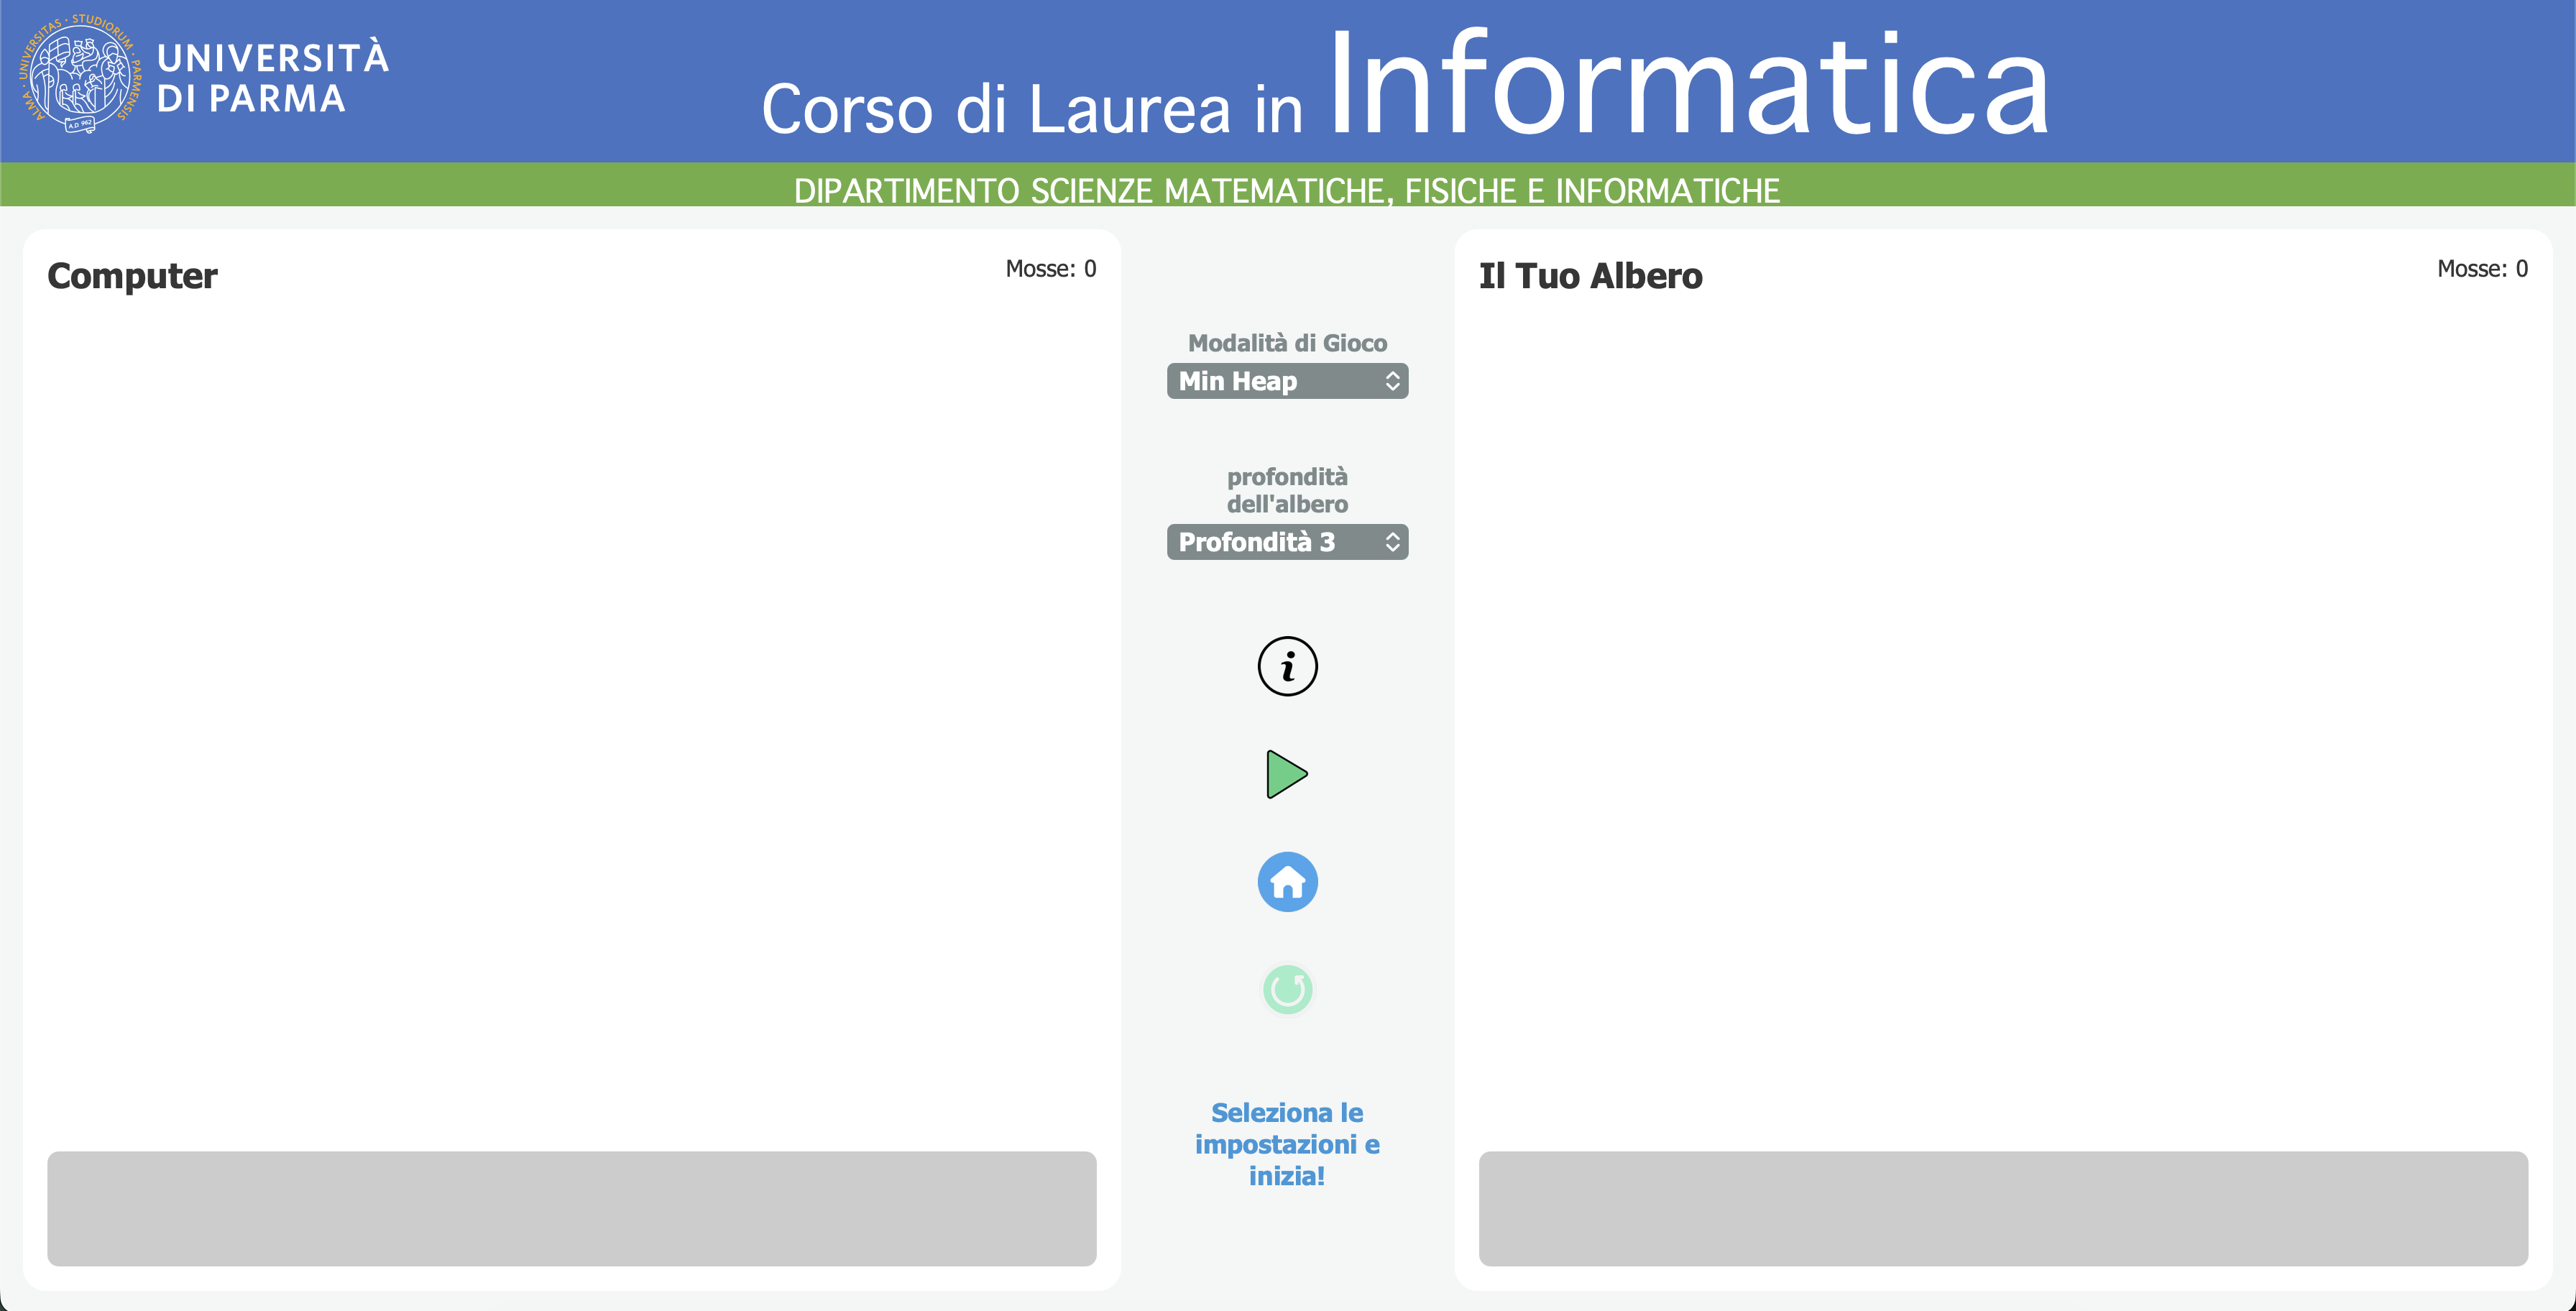
\includegraphics[width=0.9\textwidth,height=0.4\textheight,keepaspectratio]{Result_images/Result.png}
    \caption{Panoramica Generale dell'Interfaccia Web Operativa e Risultati a schermo}
    \label{fig:result_generale}
\end{figure}

\section{Configurazione e Personalizzazione}
Un elemento fondamentale dell'applicativo è la capacità di adattarsi alle diverse esigenze didattiche attraverso un pannello di controllo dedicato. Come mostrato nella Figura \ref{fig:impostazioni}, l'utente può configurare parametri chiave prima di avviare la sfida.

\begin{figure}[H]
    \centering
    
\includegraphics[width=0.7\textwidth,height=0.35\textheight,keepaspectratio]{Result_images/impostazioni.png}
    \caption{Pannello di Configurazione e Impostazioni del Gioco}
    \label{fig:impostazioni}
\end{figure}

\section{Guida all'Utilizzo}
Per agevolare l'approccio iniziale dell'utente alla sfida, l'applicativo integra una guida rapida interattiva. Come mostrato nelle Figure \ref{fig:howtoplay} e \ref{fig:howtoplay1}, queste schermate forniscono le direttive necessarie per comprendere le regole del gioco e le modalità di interazione con la struttura dati Heap.

\begin{figure}[H]
    \centering
    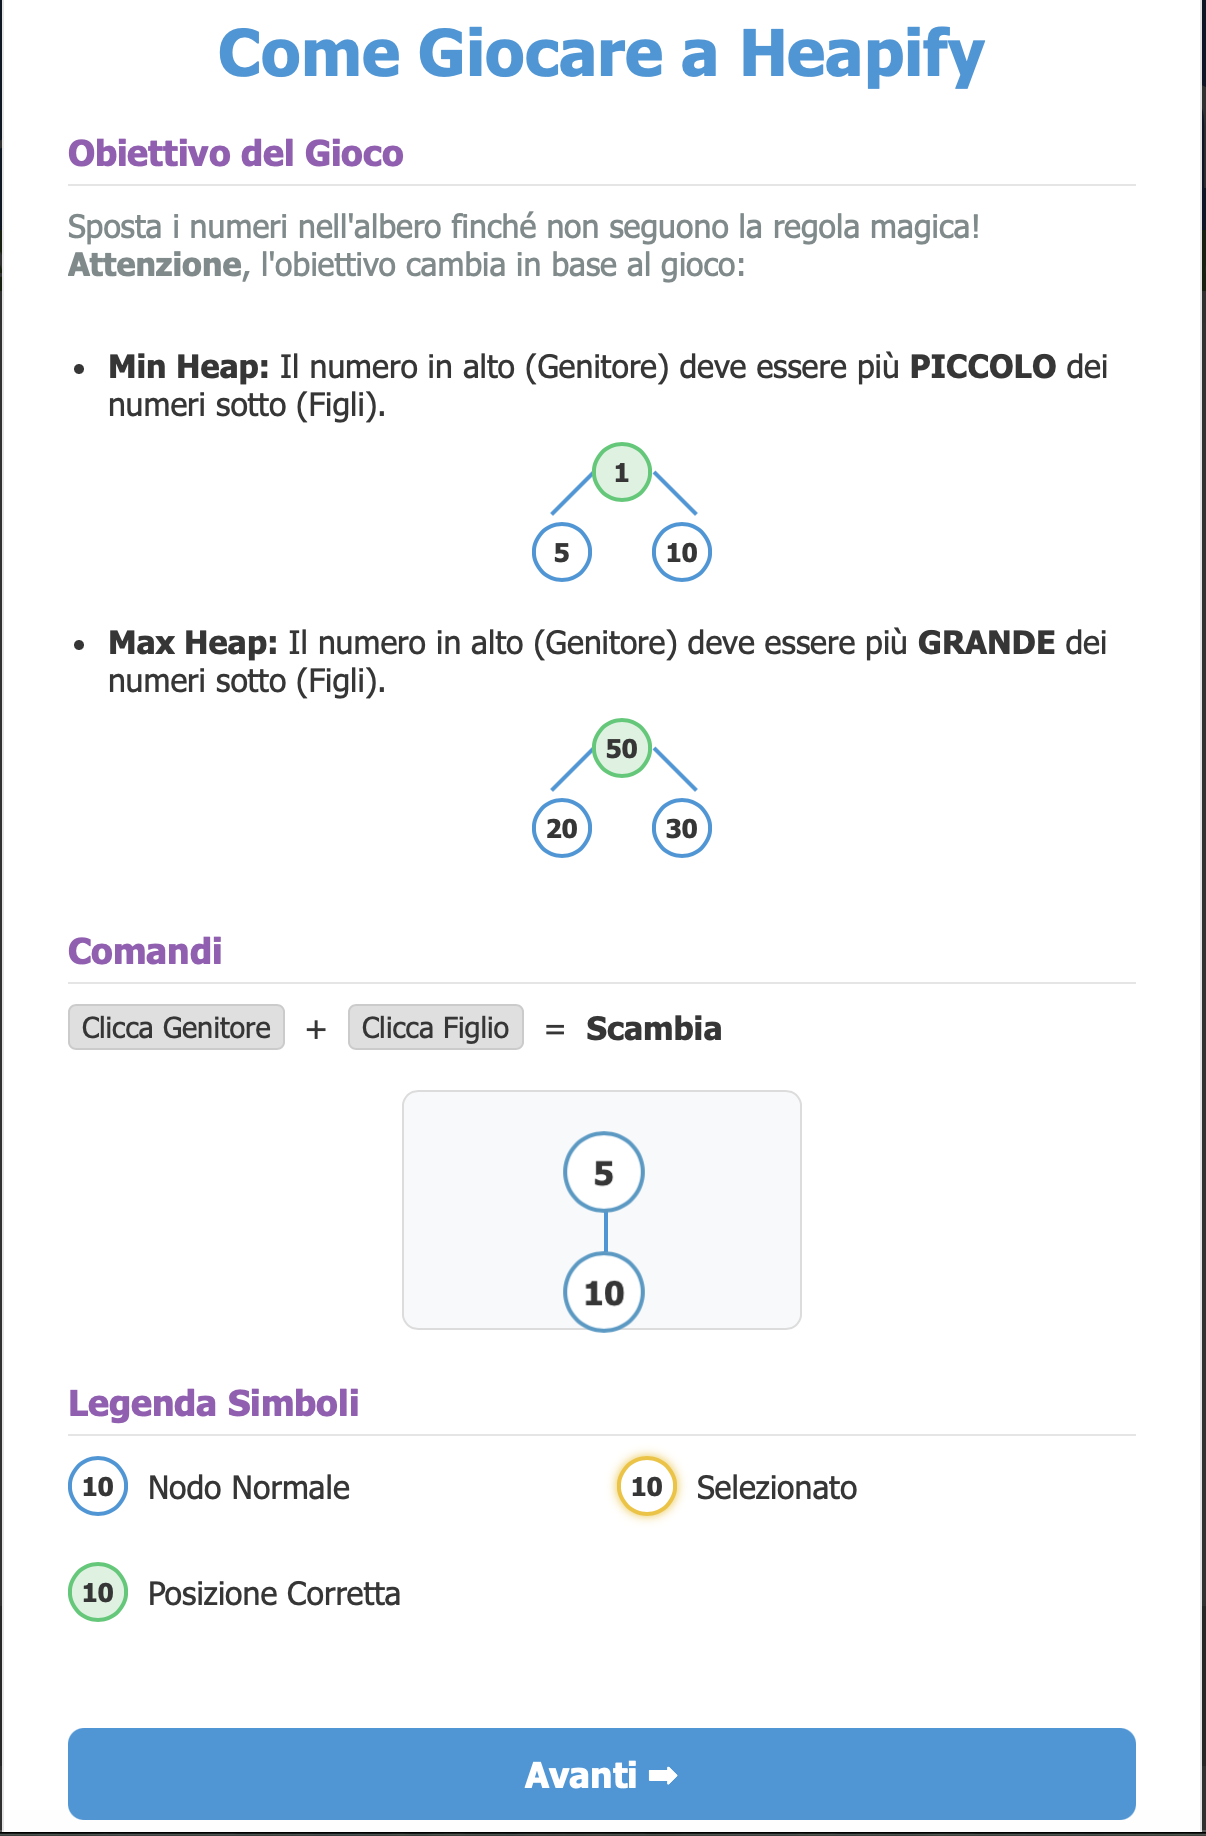
\includegraphics[width=0.7\textwidth,height=0.35\textheight,keepaspectratio]{Result_images/howtoplay.png}
    \caption{Prima parte della guida: Regole e obiettivo del gioco}
    \label{fig:howtoplay}
\end{figure}

\begin{figure}[H]
    \centering
    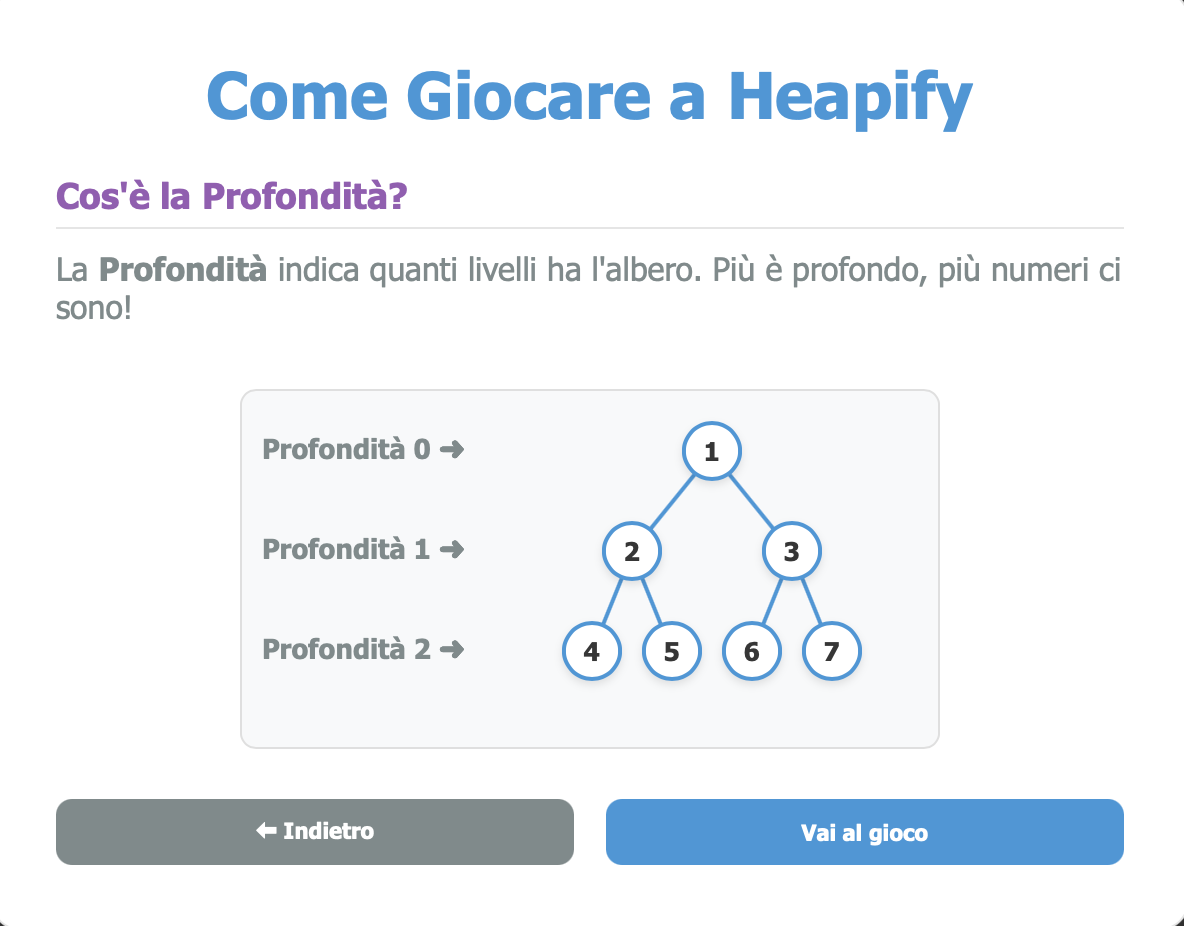
\includegraphics[width=0.7\textwidth,height=0.35\textheight,keepaspectratio]{Result_images/howtoplay1.png}
    \caption{Seconda parte della guida: Profondità}
    \label{fig:howtoplay1}
\end{figure}

\section{Avvio della Sessione di Gioco e Analisi dell'Interfaccia}
Una volta completata la configurazione iniziale attraverso il pannello centrale e consultata la guida interattiva, l'utente può avviare la sfida cliccando sull'icona di "Play". Questo momento segna la transizione critica dall'interfaccia di configurazione all'ambiente operativo di gioco. Come illustrato nella Figura \ref{fig:avviogioco}, l'interfaccia si trasforma per ospitare le strutture dati attive, organizzate secondo un layout simmetrico progettato per massimizzare la comprensione del confronto algoritmico.

\subsection{Organizzazione Visiva della Schermata}
L'interfaccia utente è stata concepita seguendo principi di ergonomia cognitiva, suddividendo lo spazio di lavoro in tre macro-aree funzionali che permettono un monitoraggio costante dell'avanzamento della sessione:

\begin{itemize}
    \item \textbf{Area Centrale di Controllo}: Posta esattamente al centro della visuale, questa colonna funge da fulcro dell'applicazione. Oltre a ospitare i selettori per la profondità dell'albero e la modalità di gioco (Min/Max Heap), presenta una serie di icone intuitive per la gestione del ciclo di vita della partita:
    \begin{itemize}
        \item \textit{Info}: Per richiamare in ogni momento la guida alle regole.
        \item \textit{Play}: Per generare un nuovo set di dati e avviare la sfida.
        \item \textit{Home}: Per navigare rapidamente verso le altre sezioni del portale didattico.
        \item \textit{Reset}: Per rimescolare i nodi mantenendo le impostazioni correnti, utile in caso di stallo logico.
    \end{itemize}
    Un elemento testuale dinamico, il \textit{Feedback di Stato}, informa costantemente l'utente su di chi sia il turno attuale o se siano state violate delle proprietà dell'heap.

    \item \textbf{Player Zone (Destra)}: Questa sezione, intitolata "Il Tuo Albero", rappresenta lo spazio d'azione diretto dell'utente. Qui l'albero binario viene renderizzato in tempo reale, con i nodi che appaiono come cerchi contenenti i valori numerici da ordinare. Sotto l'albero, una barra orizzontale rappresenta l'array di destinazione dove i numeri vengono gradualmente "estratti" e posizionati una volta che la proprietà dell'heap è stata soddisfatta per l'intero albero.

    \item \textbf{Computer Zone (Sinistra)}: Speculare alla zona del giocatore, questa area mostra l'albero gestito dall'intelligenza artificiale. La sua funzione è puramente osservativa e comparativa: l'utente può vedere come il computer risolve lo stesso problema algoritmico in tempo reale, comprendendo visivamente le euristiche di ottimizzazione utilizzate dalla macchina.
\end{itemize}

\subsection{Interazione e Feedback Dinamico}
L'esperienza d'uso si basa su un paradigma di interazione "point-and-click" estremamente semplificato ma rigoroso dal punto di vista logico. Per eseguire uno \textit{Swap} (scambio) tra due nodi, l'utente deve selezionare prima il nodo genitore e successivamente il nodo figlio (o viceversa). 

Il sistema di feedback visivo gioca un ruolo fondamentale per guidare l'utente attraverso gli stati del gioco:
\begin{itemize}
    \item \textbf{Stato di Selezione}: Quando un utente clicca su un nodo, questo cambia colore (solitamente assumendo una tonalità più scura o un bordo evidenziato), indicando che il sistema è in attesa di un secondo clic per completare l'azione di scambio.
    \item \textbf{Validazione della Posizione}: Se un nodo occupa una posizione corretta rispetto alla regola Min/Max Heap impostata (ovvero se tutti i suoi figli rispettano la gerarchia di valore), esso viene evidenziato con un gradiente verde brillante. Al contrario, se le proprietà sono violate, il nodo rimane nel suo stato neutro, segnalando implicitamente la necessità di un'ulteriore manipolazione.
    \item \textbf{Contatore delle Mosse}: In alto sopra ogni arena, un contatore digitale traccia il numero di scambi effettuati. Questo introduce un elemento di \textit{Gamification}: l'obiettivo non è solo risolvere l'algoritmo, ma farlo con il minor numero di mosse possibile, cercando di eguagliare o superare l'efficienza della CPU.
\end{itemize}

\begin{figure}[H]
    \centering
    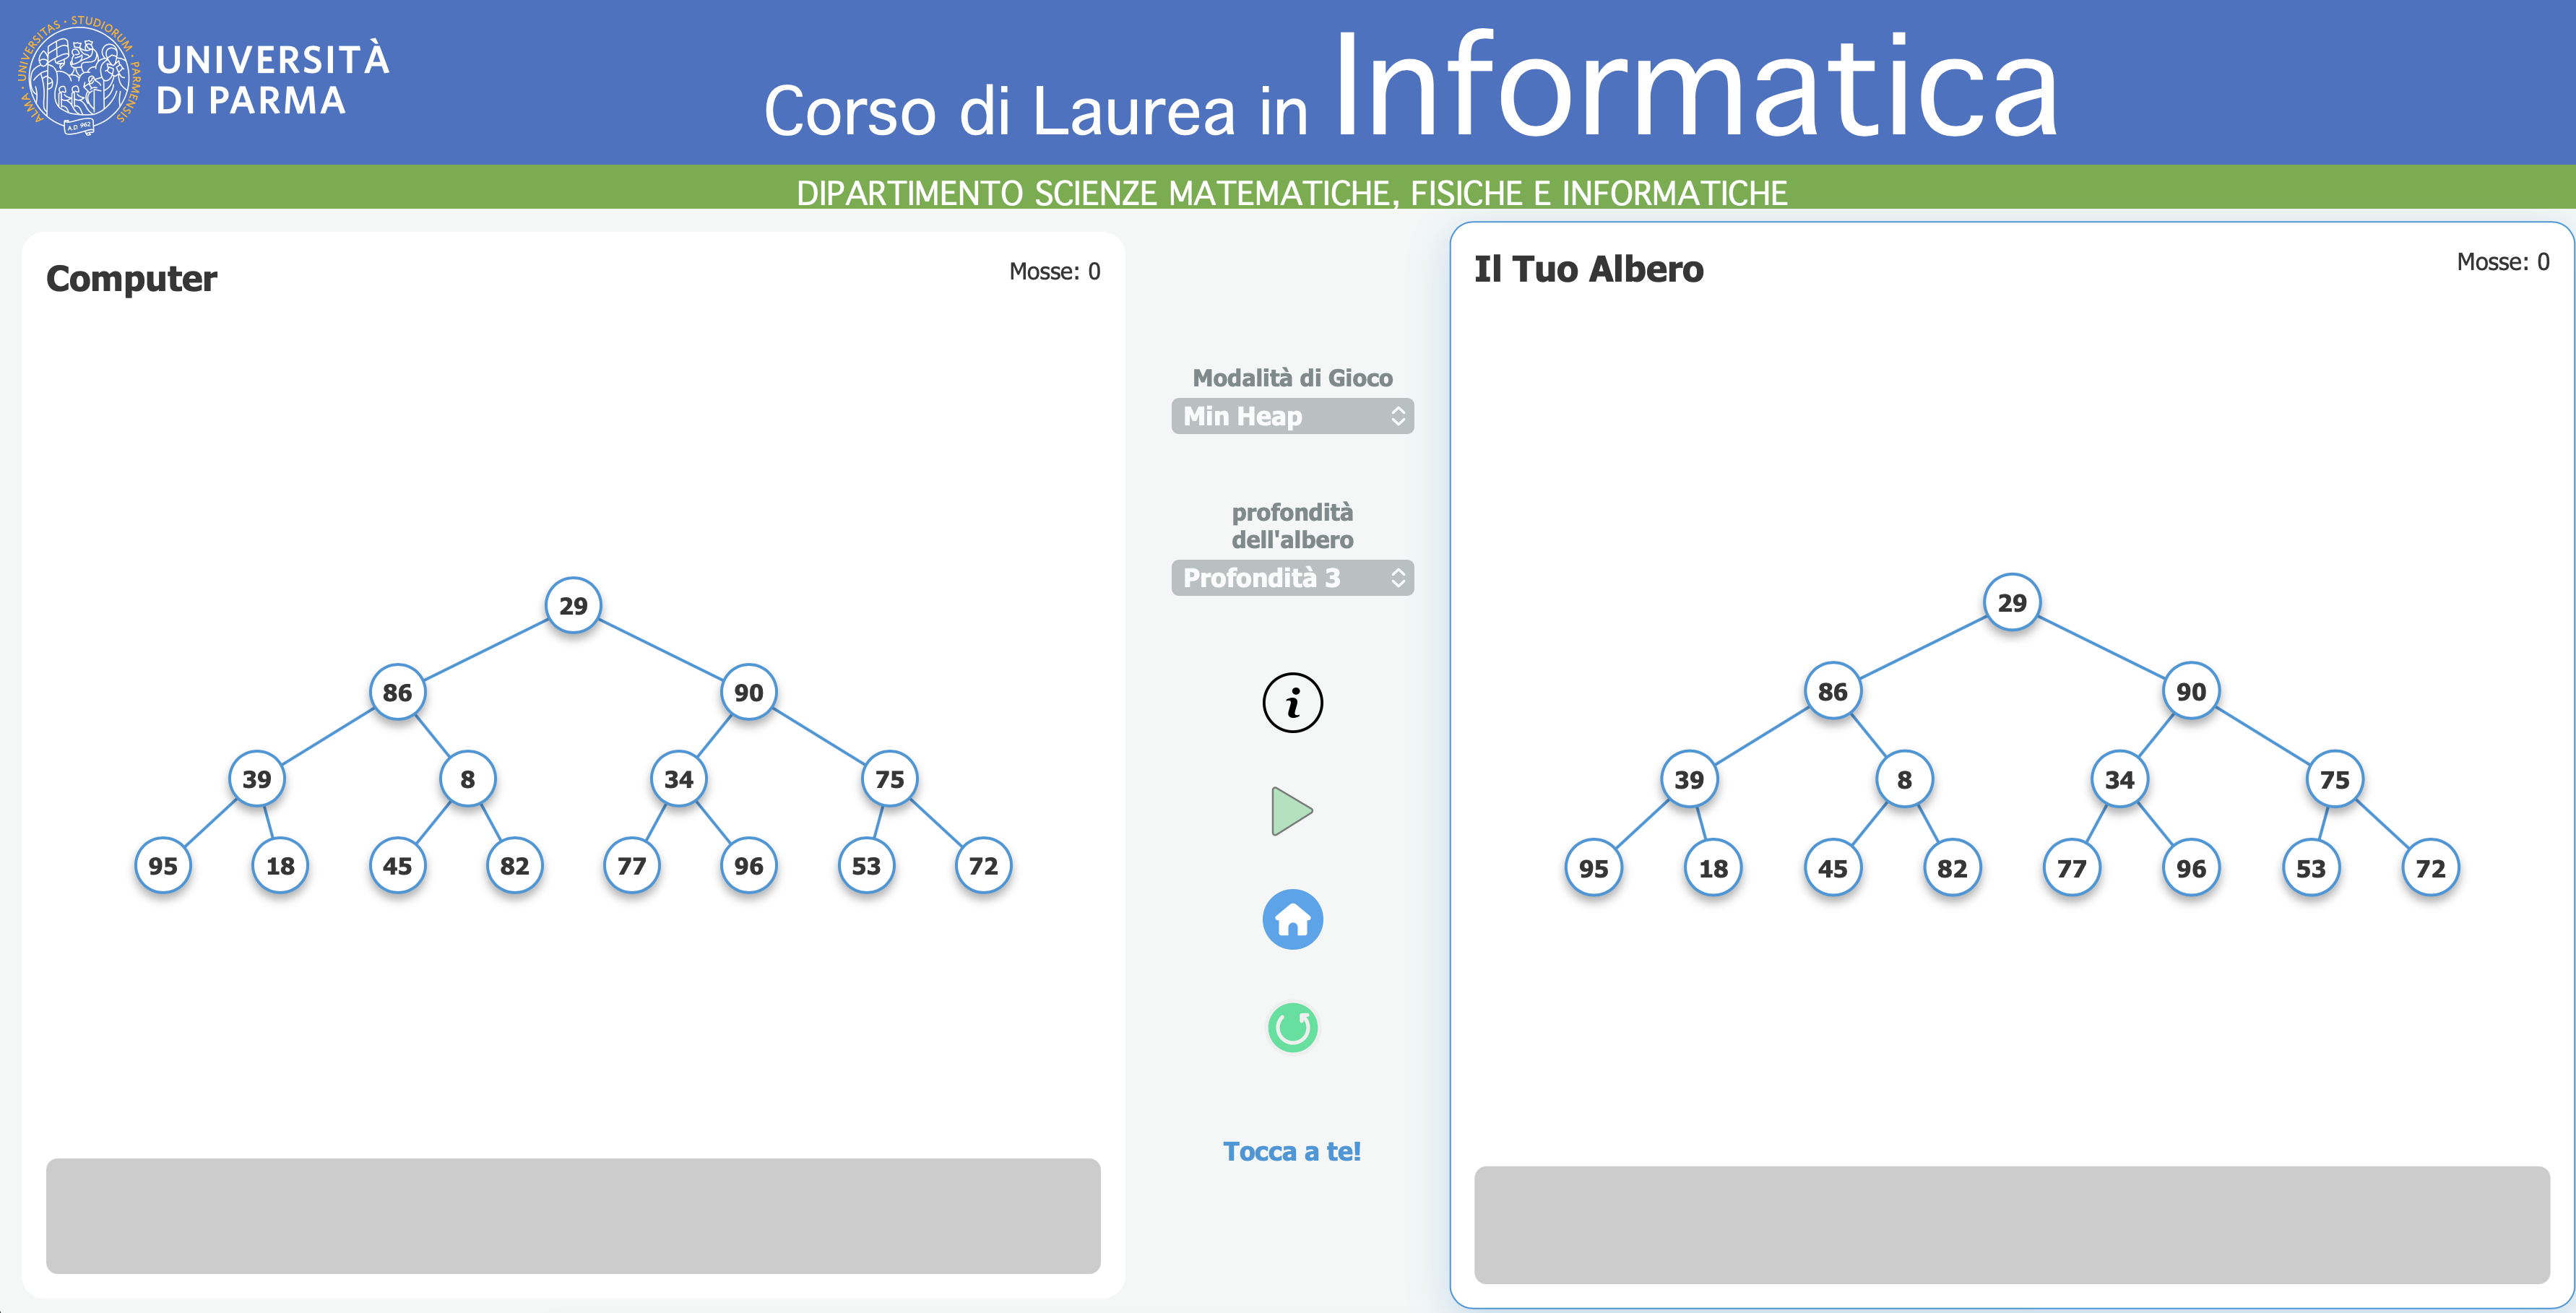
\includegraphics[width=0.9\textwidth,height=0.4\textheight,keepaspectratio]{Result_images/avviogioco.png}
    \caption{Layout operativo della sessione di gioco attiva, con evidenza del sistema di feedback visivo sui nodi.}
    \label{fig:avviogioco}
\end{figure}

\subsection{Flusso d'Uso Tipico}
Il percorso dell'utente all'interno della sessione di gioco può essere riassunto nei seguenti passaggi operativi:
\begin{enumerate}
    \item \textbf{Inizializzazione}: L'utente preme "Play". Gli alberi vengono popolati con numeri casuali non duplicati.
    \item \textbf{Analisi Visiva}: Lo studente deve scansionare l'albero partendo dai livelli più bassi (le foglie) per risalire verso la radice, individuando le violazioni della proprietà Heap.
    \item \textbf{Risoluzione Locale}: Attraverso clic successivi, i nodi vengono scambiati. Ad ogni scambio corretto, il sistema colora di verde i nodi che ora soddisfano la proprietà.
    \item \textbf{Estrazione}: Una volta che la radice contiene il valore massimo (o minimo), questa viene "estratta" e spostata nell'array inferiore, riducendo la dimensione dell'albero e avviando un nuovo ciclo di ordinamento.
\end{enumerate}
Questo ciclo si ripete fino a quando l'albero è vuoto e l'array sottostante è completamente ordinato, momento in cui appare un messaggio di vittoria che riassume le performance ottenute.

La combinazione di questi elementi trasforma una spiegazione astratta in un'esperienza multisensoriale, dove il colore, il movimento e la competizione cooperano per fissare nella memoria dello studente i meccanismi profondi dell'Heap Sort.


\section{Esito della Partita e Feedback di Fine Sessione}
Il ciclo di apprendimento si conclude con la visualizzazione di un feedback esplicito basato sulle performance dell'utente rispetto a quelle del computer. Come mostrato nelle Figure \ref{fig:vinto} e \ref{fig:perso}, il sistema utilizza dei "modali" (finestre sovrapposte) per comunicare il risultato finale in modo chiaro e coinvolgente.

\begin{figure}[H]
    \centering
    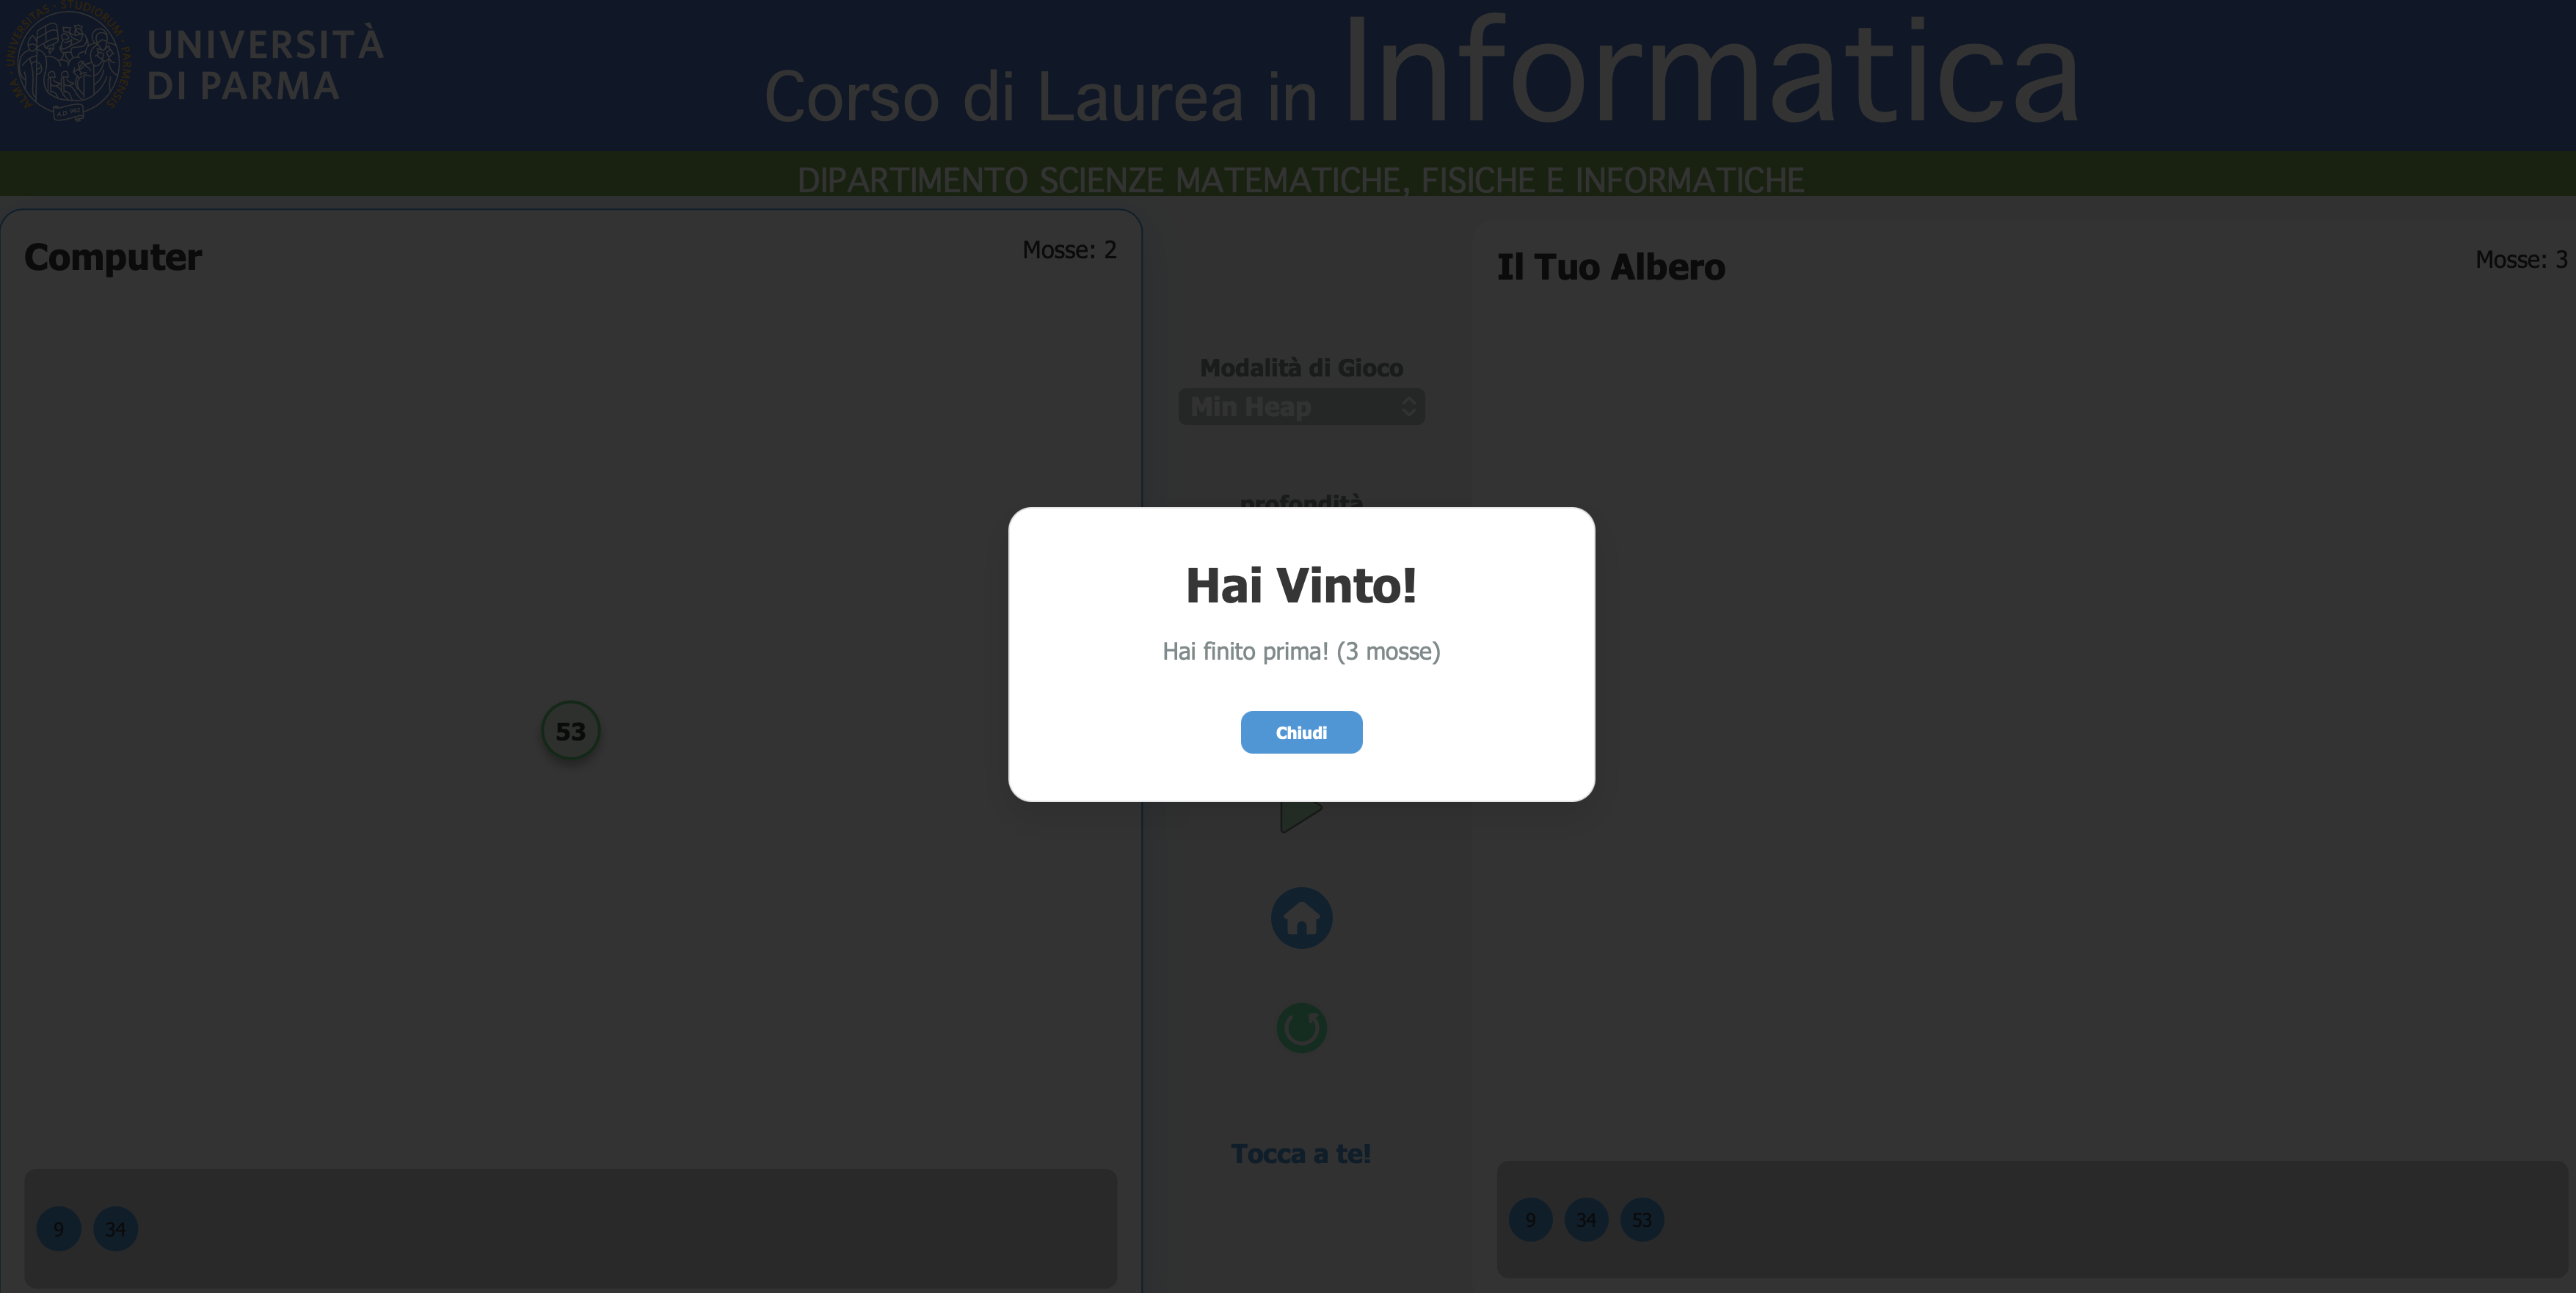
\includegraphics[width=0.8\textwidth,height=0.35\textheight,keepaspectratio]{Result_images/vinto.png}
    \caption{Messaggio di vittoria visualizzato quando l'utente completa l'ordinamento per primo.}
    \label{fig:vinto}
\end{figure}

Il messaggio di vittoria (Figura \ref{fig:vinto}) non si limita a dichiarare il successo, ma fornisce una gratificazione visiva che rinforza l'apprendimento positivo. Al contrario, in caso di sconfitta (Figura \ref{fig:perso}), il sistema incoraggia lo studente a riprovare, sottolineando che l'errore è parte integrante del processo di comprensione algoritmica.

\begin{figure}[H]
    \centering
    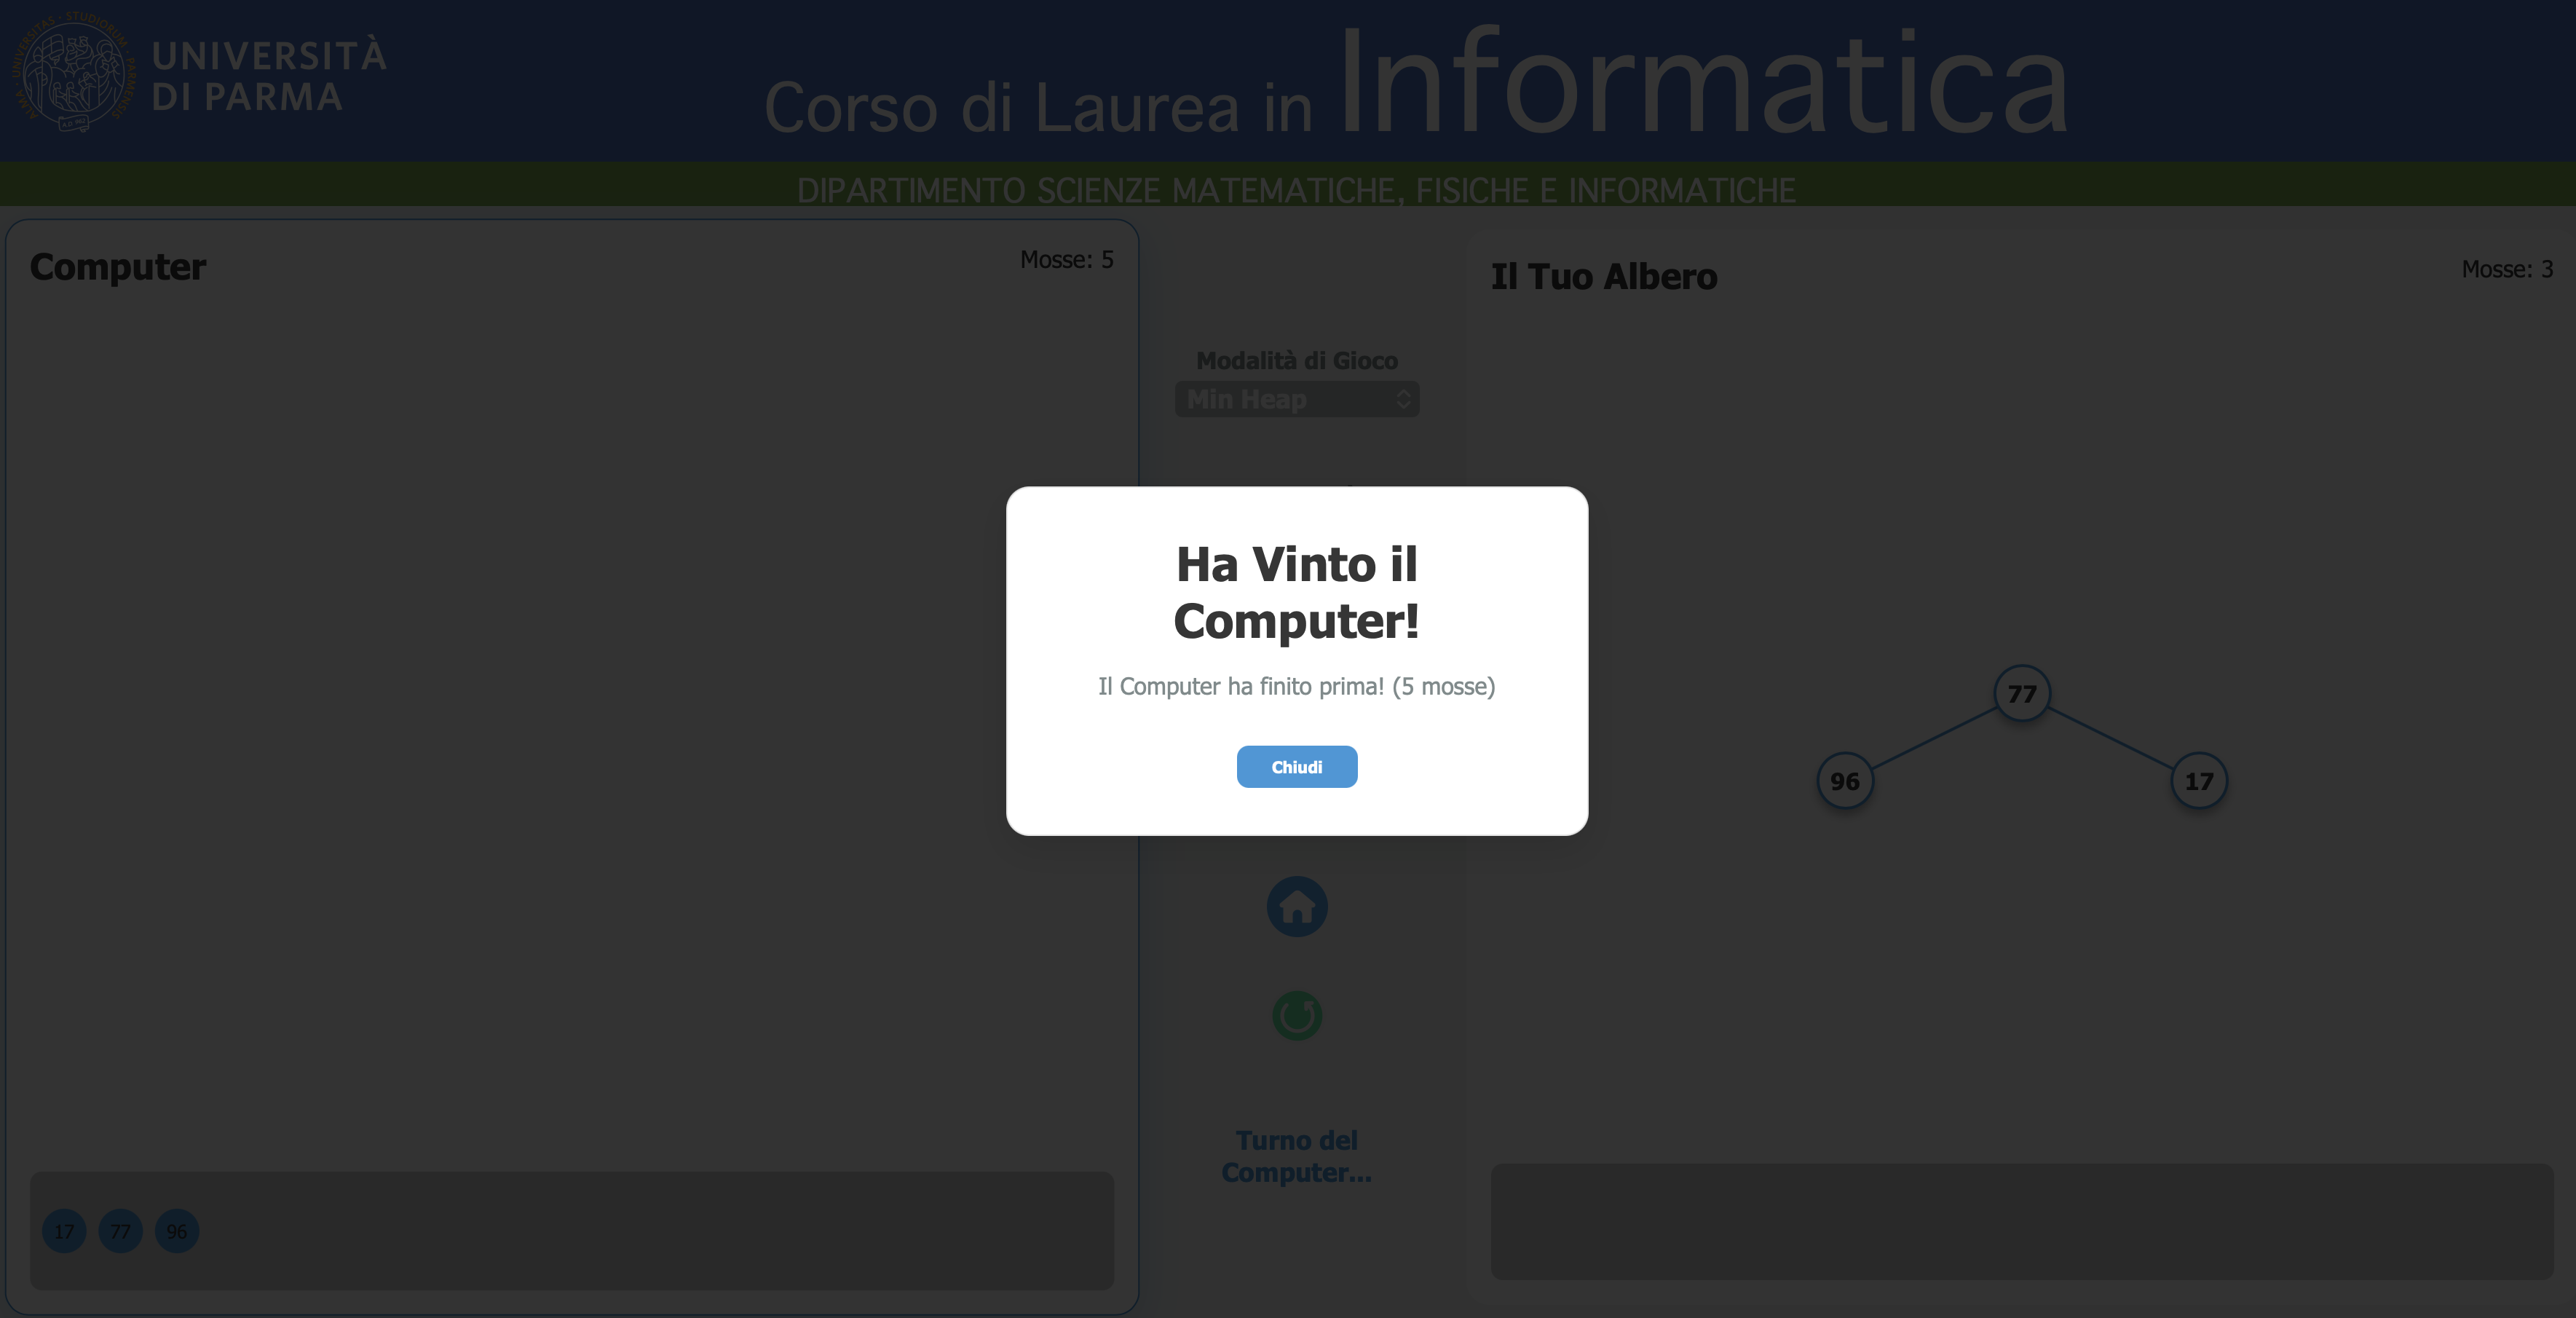
\includegraphics[width=0.8\textwidth,height=0.35\textheight,keepaspectratio]{Result_images/perso.png}
    \caption{Messaggio di sconfitta visualizzato in caso di performance superiore della CPU.}
    \label{fig:perso}
\end{figure}

\chapter*{Conclusioni}
\addcontentsline{toc}{chapter}{Conclusioni}

Il percorso di sviluppo intrapreso in questo progetto di tesi ha permesso di trasformare una sfida puramente algoritmica in un'applicazione didattica interattiva moderna e performante. L'obiettivo primario — ovvero l'abbattimento della barriera di astrazione tipica dello studio delle strutture dati lineari e non lineari — è stato perseguito attraverso la fusione di rigore logico, architettura software solida e principi di gamification.

\section*{Riflessioni Tecniche e Architetturali}
Dal punto di vista dell'implementazione, la scelta di adottare il pattern \textbf{Model-View-Presenter (MVP)} si è rivelata determinante. Questa separazione netta delle responsabilità ha garantito che la logica matematica dell'Heap Sort (il Model) rimanesse incontaminata dalle necessità di visualizzazione (la View), permettendo al Presenter di agire come un orchestratore fluido e facilmente manutenibile.

L'utilizzo di tecnologie standard come \textbf{HTML5, CSS3 e Vanilla JavaScript (ES6)}, senza l'ausilio di framework esterni pesanti, ha dimostrato come sia possibile ottenere una manipolazione del DOM ad alta efficienza e una reattività visiva eccellente anche per strutture dati complesse come i grafi bidimensionali. La gestione manuale delle transizioni e delle posizioni assolute dei nodi tramite coordinate polari e cartosiane ha conferito al software un carattere distintivo di "leggerezza" e velocità di caricamento, critiche in contesti educativi online.

\section*{L'Approccio Pedagogico: Gamification e Visualizzazione}
L'integrazione di elementi ludici ha trasformato l'apprendimento in un'esperienza competitiva e coinvolgente. La possibilità di sfidare un'intelligenza artificiale asincrona non solo stimola l'interesse dello studente, ma offre un termine di paragone oggettivo sull'efficienza delle proprie scelte algoritmiche. Il sistema di feedback visivo basato sul colore (verde per la correttezza, evidenziazione per la selezione) agisce come un tutor silenzioso che guida l'utente verso la risoluzione corretta del problema, riducendo la frustrazione derivante dall'errore cieco.

L'esperienza ha confermato che la rappresentazione grafica dinamica di un array sotto forma di albero binario permette di interiorizzare i concetti di "parent-child relationship" in modo quasi intuitivo, rendendo immediata la comprensione di operazioni complesse come lo \textit{Sift-Up} e lo \textit{Sift-Down}.

\section*{Traguardi Raggiunti e Competenze Acquisite}
Lo sviluppo di questo applicativo ha rappresentato una sfida significativa non solo tecnica, ma anche metodologica. È stato necessario trovare un equilibrio costante tra la precisione matematica richiesta dall'algoritmo e l'estetica necessaria per un'interfaccia utente premium. Il superamento di ostacoli quali la prevenzione dei duplicati nella generazione dei nodi, la gestione dei turni asincroni e la sincronizzazione millimetrica dei grafi rispetto all'array logico ha contribuito a una crescita professionale profonda nell'ambito del web development moderno.

Il progetto finale si presenta quindi come uno strumento maturo, capace di coprire l'intero spettro didattico: dalla teoria pura alla pratica interattiva, fino alla valutazione delle performance.

\section*{Sviluppi Futuri e Prospettive}
Sebbene l'attuale versione del software sia completa e funzionale, il framework architetturale creato è intrinsecamente scalabile. In futuro, il sistema potrebbe essere esteso per includere:
\begin{itemize}
    \item \textbf{Nuovi Algoritmi}: L'implementazione di Quick Sort o Merge Sort seguendo la stessa logica visiva.
    \item \textbf{Multiplayer Online}: Una vera sfida 1vs1 tra utenti connessi in rete tramite WebSocket.
    \item \textbf{Analisi Statistica Avanzata}: Un pannello per il docente capace di tracciare i tempi medi di risoluzione e le difficoltà riscontrate dagli studenti.
    \item \textbf{Supporto Mobile}: Un'ottimizzazione dell'interfaccia per il completamento delle sfide su dispositivi touch.
\end{itemize}

In conclusione, questo lavoro dimostra che l'informatica educativa può e deve evolversi verso strumenti che non solo spiegano "come" funziona un sistema, ma permettono di "vivere" la logica che lo sottende. L'informatica è, per sua natura, una disciplina dinamica; è giusto che anche il modo di insegnarla rifletta questa vitalità, ponendo lo studente al centro di un ecosistema digitale interattivo, stimolante e, soprattutto, gratificante.

\bibliographystyle{apalike}
\nocite{*}
\clearpage
\phantomsection
\addcontentsline{toc}{chapter}{Bibliografia}
\renewcommand{\bibname}{Bibliografia}
\bibliography{Bibliografia}

\clearpage
\chapter*{Ringraziamenti}
\addcontentsline{toc}{chapter}{Ringraziamenti}

Desidero esprimere la mia più sincera gratitudine al \textbf{Prof. Vincenzo Bonnici}, relatore di questa tesi, per avermi guidato con professionalità e disponibilità lungo tutto questo percorso. Il suo supporto è stato fondamentale non solo nella fase di ricerca, ma soprattutto nello sviluppo del progetto, dove le sue indicazioni e i suoi consigli hanno fatto la differenza. La sua passione per l'informatica mi ha ispirato e motivato a dare il massimo in questo lavoro.

Un ringraziamento speciale va a tutti i \textbf{docenti} che ho incontrato durante il mio percorso universitario. Le loro lezioni, la loro disponibilità e i loro consigli sono stati essenziali per la mia crescita personale e professionale, fornendomi le basi e la motivazione necessarie per portare a termine questo percorso.

Vorrei inoltre ringraziare di cuore i miei \textbf{amici e colleghi di corso}, che mi hanno incoraggiato e sostenuto con entusiasmo. Il loro aiuto nello studio, la loro compagnia e la loro capacità di motivarmi nei momenti di difficoltà hanno reso questo cammino più leggero e stimolante. La loro presenza nei periodi più complessi è stata fondamentale per trovare la forza e la determinazione necessarie a raggiungere questo importante traguardo.

Infine, il mio più sentito ringraziamento va a tutta la mia \textbf{famiglia}, in particolare a mia madre \textbf{Ticho Bernadette} e alla famiglia \textbf{Yewo}, che mi ha sempre sostenuto con amore e pazienza durante tutto il percorso universitario. Un grazie speciale va a \textbf{Yewo Simo Henri Claudel}, \textbf{Wadeu Ngaffi Viviane}, \textbf{Yewo Simo Serena}, \textbf{Yewo Simo Noemi}, \textbf{Yewo Simo Cindy Djoumu} e, con tutto l'affetto del mio cuore, alla piccola \textbf{Yewo Simo Cloé}. La loro vicinanza, il loro supporto e i loro consigli sono stati determinanti per superare le difficoltà e completare con successo questo percorso di studi.

\bigskip
\noindent A tutti voi, il mio più sincero grazie.

\end{document}
